\documentclass{my_paper}
\usepackage{ctex}
\usepackage[textwidth=444bp,vmargin=2.5cm]{geometry}%设置页边距
\usepackage{array} %主要是增加列样式选项
\usepackage[dvipsnames]{xcolor}%颜色宏包
\usepackage{graphicx}%图片宏包
\usepackage{amsmath}%公式宏包
\usepackage[T1]{fontenc}    
\usepackage{newtxtext, newtxmath}  %两种使用Times New Roman 字体的方法
\usepackage{subfigure}
\usepackage { gensymb }
% 打°符号\degree
\usepackage{listings}
% 代码
\usepackage{tabularx, booktabs} %% Load packages that you use
\usepackage{multirow} %跨行处理
\usepackage{rotating}%横向表格
\usepackage{diagbox}%斜线划分表头
\begin{document}

\newpage
\begin{center}
\lunwenbiaoti

\vspace{2ex}
\zhaiyao
\end{center}

本文针对Tacview战斗复盘问题,使用决策树,双重滑动窗口,熵权法等多种知识,得出飞机各个时刻的动作序列,分析出各个时刻飞机动作意图,在此基础上分析了子动作序列的意图并进行了战场的势态评估。

针对飞机动作描述和量化问题,我们查阅资料并结合附件中所给数据信息,列举九种基本动作及其飞行参数变化趋势。建立决策树对给定的飞行参数组合进行识别,确定该时刻的飞行动作。

针对飞行动作序列识别问题,我们利用双重滑动窗口和相关阈值的确定来将具体数值转换为定性的评价,建立了参数值(定量)和飞行动作的区分因素(定性)的关系。其中趋势识别等阈值的确定均由飞行数据中的均值方差等统计量得出,个别阈值由查阅相关文献获得。使用双窗口法判断飞行参数序列变化趋势,能够有效消除噪声并捕获趋势,得到飞行参数趋势序列,再利用问题一中建立的模型,有效确定了飞行动作序列,并按指定格式输出了动作序列。

针对动作子序列划分及意图识别问题,我们先由战场情况建立意图识别模型。我们就发射导弹的飞机与最近敌机的距离统计量确定了战备距离,就该距离划分敌机是否属于战斗意图。在细分战斗意图的过程中建立了角度、高度、距离和速度四个优势函数,并通过熵权法将四个函数合并为一个总体优势函数,以此来作为战斗中敌我双方优势的衡量指标,从而判断细分的战斗意图。在战斗意图识别完成后,将战斗意图和相应时间的动作序列对应,即得到动作序列按意图的划分。

针对战场势态分析,我们在第三问的基础上,将单个飞机的优势函数以相加形式拓展到整个联盟,并引入了干扰弹的影响,得到联盟整体的优势函数。以双方优势函数值的比重作为战胜概率,由此建立了整体势态评估模型。在模型建立后使用一场战役验证战场态势模型,并分析了其含义。

该模型具有动作覆盖全面,动作意图和势态识别准确等特点,对不同的战斗场景均有较好效果,有较大应用价值。

\begin{guanjianci}

 决策树 \quad 双重滑动窗口 \quad 熵权法
\end{guanjianci}

%----------- 正文 ----------
%----------- 一、问题重述 ----------
\newpage
\section{一、问题重述}

随着空战游戏越来越吸引玩家的目光,游戏开发过程中如何设计良好的人机交互工作,已经成为一项具有挑战性的工作。

在游戏中玩家操纵飞机,在飞机的机动性能约束下实现各种各样的战斗机动动作,实现各种各样的策略以及完成意图。分析调研飞行数据,可以帮助团队评估格斗行为的效果和玩家的飞行水平,从而进行改进。

经过分析整理,我们需要解决以下问题:
\begin{enumerate}
    \item 通过有关文献研究飞机的机动动作,建立尽可能完善的机动动作描述与量化模型。
    \item 通过附件中的10场飞机时序数据,得到每架飞机的飞行动作序列,按指定格式输出。
    \item 建立机动序列的动作分割算法,判断各个动作子序列的意图,并利用附件中数据进行验证。
    \item 建立空战态势评估模型,利用附件中数据进行验证。
\end{enumerate}
\section{二、问题分析}
\subsection{问题一的分析}

该问要求我们查阅参考资料,建立战机机动的量化模型。为此考虑根据已知的飞行参数确定对应的战斗机机动行为。一个战斗行为可能对应一系列参数的变化,因此结合多个参数的变化情况来判断动作类型,对于某些复杂动作,可能会有多段变化过程,因此需要结合相邻的两次变化情况进行判断。由于决定飞机飞行动作的参数种类有限,每一种参数也只有集中情况,考虑就飞行参数变化建立决策树,对战斗机的机动行为进行识别。

\subsection{问题二的分析}

分析题中附件所给数据,得出附件中信息有以下特点:数据冗余、数据缺失和个体多样问题。针对数据冗余问题,需要去除那些不便于利用的数据格式;针对数据缺失问题,需要采用缺失处相邻部分的数据进行填充,考虑到填充过程不应当引入噪声,因此采用matlab工具箱中的移动均值方法填补缺失数据;对于数据个体多样问题,由于每个个体的动作分析应当独立进行,且需要分析的个体类型为“Air+FixedWing”且每次战斗不止有一架飞机参与战斗,因此需要使用id和类型对时间序列进行分类分析。

在分析数据的基础上,我们还构思了提取飞行参数变化情况的方法。单一飞机一段时间内的飞行数据,可以看作是多维度的时间序列数据。为了分析各个维度的变化状态,尝试使用差分法,但是体现出易受噪声干扰和局部性的特点,不能很好体现出数据的变化趋势。由于以上原因,又改用双滑动窗口法,具有较好的消除噪声和判断趋势的能力。

\subsection{问题三的分析}

要推知战场上战斗机的动作序列意图,我们仅仅使用飞机战斗动作序列是不够的。这是由于模拟战斗过程中状况千变万化,同一战斗动作可能在不同的战斗过程中体现不同的意图。因此需要先结合战场真实情况,包括敌我双方的战机与导弹位置分布与方位角指标等信息来分析战场情况。随后将战场情况数据通过决策手段来判断战机意图。在将意图所对应的时间区间内的动作状态和该意图之间进行对应。通过分析一场战役中的某些意图对应的动作序列,分析其统计特征,最后分析出子动作序列和意图之间的关系。

\subsection{问题四的分析}

战场态势由战场上属于阵营内的一类飞机所构成,因此每架战机的意图和该阵营的态势关系密切相关。分析附件数据,由于战场上存在干扰弹,可能会对战斗评价函数带来整体干扰。故考虑整体态势时应当将其考虑其中。对比双方整体态势的大小可以推断出获胜的概率。

%----------- 三、模型假设 ----------
\section{三、模型假设}
%使用代码片段:、jiashe%
\begin{enumerate}
    \item 飞机所记录的飞行参数真实可信,没有因各种因素而导致数据错误。
    
    \textbf{原因:}动作序列的分割识别工作基于飞行时的各项参数所决定,如果飞行参数有误,那么所计算得出的动作序列将不准确。

    \item 飞机的作战意图只针对最近的对方飞机而言。
    
    \textbf{原因:}在飞机作战时对于最近的敌机进行追逐攻击最为经济和高效,且这样考虑简化了计算。
    
    \item 一方导弹出现时离其最近的同盟机为发射该导弹的飞机,离同盟飞机最近的敌军飞机是导弹的攻击目标。
    
    \textbf{原因:}附件中包含的数据并未指明导弹由哪架飞机发射而出,故按发射时距离最近的飞机和导弹相联系。同理,附件中导弹数据缺失方位角,无法推知其指向的目标。就可行性而言,原始数据在时间维度上采样频率足够高,导弹刚从飞机上发射时相关参数即可被记录。
\end{enumerate}

%----------- 四、符号说明 ----------
\section{四、名词解释与符号说明}
%使用三线表格最好~
\subsection{名词解释}
\begin{enumerate}
    % 名词:、mingci
    \item \textbf{飞行参数}
    
    在空战模拟中飞机的时序数据,包含飞机海拔高度,真实空速(TAS),俯仰角,偏航角(Yaw)等指标。每条指标由id与Unix时间唯一标识。
    
    \item \textbf{机动动作}
    
    战机在空中飞行过程中,飞机为了某些战术意图而做出的行为。在分析过程中,机动动作是最小的分析单位,不能再进行分割。

    \item \textbf{意图}
    
    查阅参考文献\cite{11}可知,在军事领域,目标意图包括两层含义:第一层指战场目标将来可能的行为,即意图决定了目标行动的选择;第二层是指目标试图完成的任务,即意图是以作战目的引导的目标行为。在这里我们采用第二种解释,飞机动作序列的执行最终目的是,这些任是实现作战意图,包括攻击,侦察等。

    \item \textbf{势态}
    
    在战斗过程中,认为一方战斗的获胜可能为势态。空战势态同全局状况密切相关,代表了敌我双方战胜或失败的可能,使用概率来度量。
    
    
\end{enumerate}
\subsection{符号说明}
以下是本文使用的符号以及含义:
\begin{table}[h]%htbp表示的意思是latex会尽量满足排在前面的浮动格式,就是h-t-b-p这个顺序,让排版的效果尽量好。
    \centering
    \begin{tabular}{p{2.0cm}<{\centering}p{9.0cm}<{\centering}p{2.0cm}<{\centering}}
 %指定单元格宽度, 并且水平居中。
    \hline
    符号 & 说明 & 单位 \\ %换行 
    \hline
    $h$ & 飞机飞行高度 &  $m$\\
    $\dot{h}$ & 飞机飞行高度变化 &  $m/s$\\
    $\alpha$ & 飞机航向角 &  $\degree$\\
    $\dot{\alpha}$ & 飞机航向角变化率 &  $\degree/s$\\
    $v$ & 飞机飞行速度 &  $m/s$\\
    $Y$ & 飞机飞行意图 &  /\\
    $M$ & 飞机飞行动作 &  /\\
    $\delta$ & 导弹发射离轴角 & \degree \\
    
    \hline
    \end{tabular}
\end{table}

%----------- 五、模型的建立与求解 ----------
\section{五、模型的建立与求解}

以下将对提出的四个问题进行建模求解。

\subsection{机动动作描述与量化模型}

为了进行空战势态感知,机动决策,意图识别等工作,常常根据需要预先建立空战动作库\cite{1}。常见的空战库设计有两种方法,分别是包含丰富战术动作的典型战术动作库和由美国NASA学者\cite{2}提出的基本操纵动作库。前者内容丰富,但是前一种方法存在识别困难,对于某些复杂动作可能中断的情况处理不佳,而后一种方式以极限情况操作粗猛,不能保证组合出所有的战术动作。文献\cite{3}中提出的机动动作集合兼顾二者的优点,列举了仪表动作,简单特技,复杂特技共三类十二种动作,如表(\ref{dongzuo}) 。这一选择兼顾了简单动作与复杂动作,具有飞行动作代表性,易于识别。

\begin{table}[h]%htbp表示的意思是latex会尽量满足排在前面的浮动格式,就是h-t-b-p这个顺序,让排版的效果尽量好。
    \centering
    \caption{战斗机的三类机动动作}
    \vspace{10pt}
    \begin{tabular}{p{4.0cm}<{\centering}p{4.0cm}<{\centering}p{4.0cm}<{\centering}}
 %指定单元格宽度, 并且水平居中。
    \hline
    仪表动作 & 简单特技 & 复杂特技 \\ %换行 
    \hline
    盘旋 & \multirow{2}*{半滚倒转} & \multirow{2}*{“S”形急转} \\
    急跃升 &  &  \\
    俯冲 & \multirow{2}*{斤斗} & \multirow{2}*{战斗转弯} \\
     水平匀速直线飞行&  &  \\
     水平加速直线飞行& \multirow{2}*{半斤斗翻转} & \multirow{2}*{眼镜蛇机动} \\
     水平减速直线飞行&  &  \\

    \hline
    \end{tabular}
    \label{dongzuo}
\end{table}


下面分别介绍各个动作的战机移动特点,并总结出各个动作的定性判别标准。
\begin{enumerate}
    \item \textbf{盘旋}
    
    据有关文献\cite{4},盘旋动作时,飞机的航向角一定会发生变化。航向角变化是盘旋的主要特点,根据航向角的变化趋势,还可以将盘旋进一步细分为左盘旋和右盘旋。此外,盘旋还可以被分为各种细类,但是考虑到识别的效率和复杂度,本文中仅考虑水平稳定盘旋,在此过程中,飞机飞行速度和飞行高度俱不变。

    \item \textbf{急跃升}
    
    在急跃升动作中,飞机迅速拉起,以达到躲避敌机和占据有利地位的目的。其飞行参数特点是提升高度的同时降低了速度。
    \item \textbf{俯冲}
    
    飞机进行俯冲动作时以大角度和高速度下冲,在飞机高度下降过程中飞机的势能转变为机械能,速度增加。
    \item \textbf{直线飞行}
    
    飞行过程中高度和方位角不发生变化,此时飞机进行直线飞行。根据加速度分为加速、匀速和减速直线飞行三种。

    \item \textbf{半滚倒转}
    
    据参考文献显示\cite{5},半滚倒转是一种常用在脱离空战情况下的机动方式。在进行该动作时,飞机先横滚半圈,再做半个内斤斗,随后在低高度下反方向改平飞出,如图(\ref{dz}a) 。该机动方式迅速改变航向的同时,降低了高度,提升速度,是一种高效的脱离方式。

    \item \textbf{斤斗}
    
    在斤斗过程中,飞机由水平直线飞行过程中拉起机身,在竖直方向上做一个圆周运动,飞机机盖指向圆周内部,如图(\ref{dz}b)。飞行参数表现为高度先升高后降低,航向角发生两次突变,速度先增后减。

    \begin{figure}[htbp]
        \centering  %居中
        \subfigure[半滚倒转示意图]{   %第一张子图
        \begin{minipage}{0.4\textwidth}%大小总和超过textwidth则自动换行
        \centering    %子图居中
        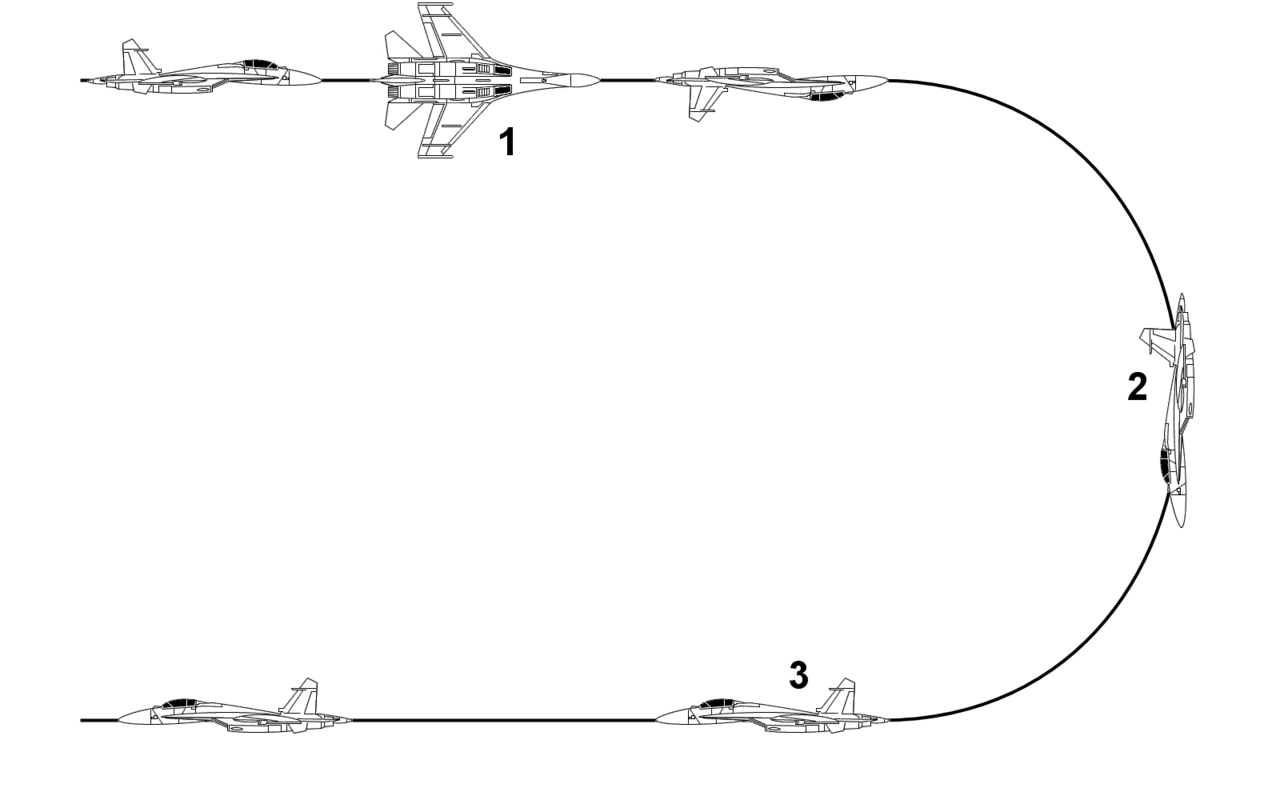
\includegraphics[width=\textwidth]{bangun.png}  %设置图片的输出大小倍数,这里是0.5倍大小输出
        \end{minipage}
        }
        \subfigure[斤斗示意图]{ %第二张子图
        \begin{minipage}{0.4\textwidth}
        \centering    %子图居中
        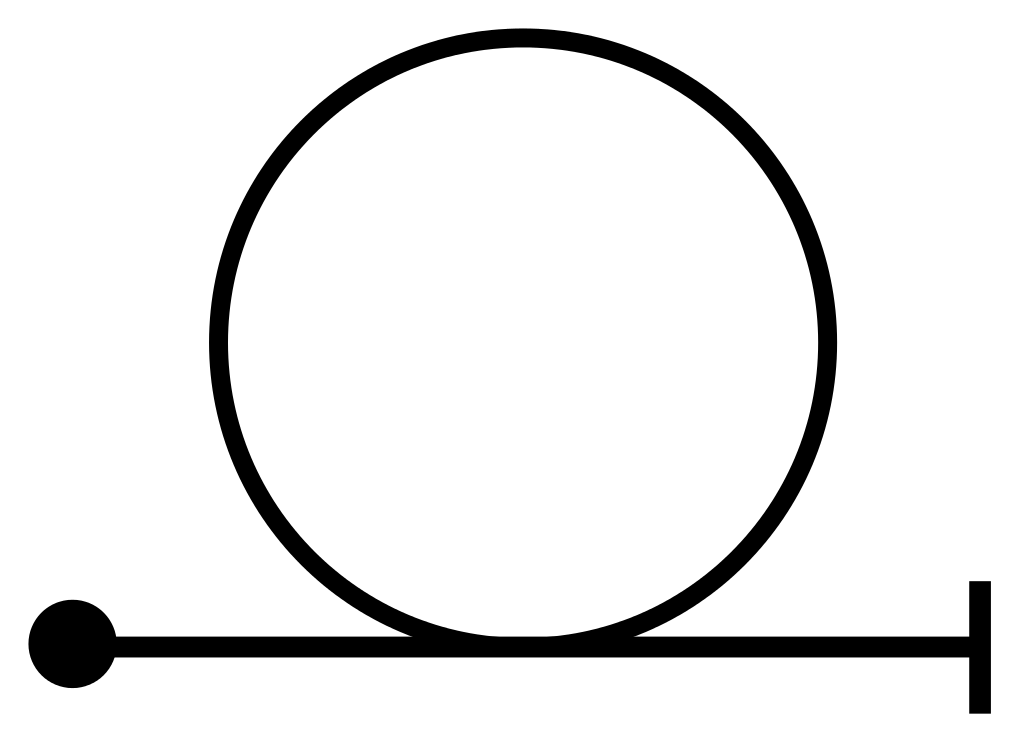
\includegraphics[width=\textwidth]{jindou.png}%以pic.jpg的0.5倍大小输出
        \end{minipage}
        }
            \subfigure[眼镜蛇机动示意图]{   %子图
            \begin{minipage}{0.4\textwidth}%大小总和超过textwidth则自动换行
            \centering    %子图居中
            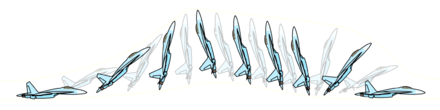
\includegraphics[width=\textwidth]{yjs.png}  %设置图片的输出大小倍数,这里是0.5倍大小输出
            \end{minipage}
            }        
    
        \caption{部分飞行动作示意图}    %大图名称
        \label{dz}    %图片引用标记
    \end{figure}
    
    \item \textbf{“S”形急转}
    
    飞机在进行“S”形急转时方向变化两次,高度不发生变化。经过该动作后的飞机航向改变。

    \item \textbf{战术转弯}
    
    该动作适用于在俯冲攻击后改出的情况,在拉升的过程中同时改变方向角。在此过程中,高度上升,方向角增加或者减少。

    \item \textbf{眼镜蛇机动}
    
    在敌机紧追我方时使用该动作对敌方进行战术躲避。\cite{7}该动作上拉机头,导致飞行速度迅速降低,随后机头开始下沉时,加大油门直到飞机转为水平姿态。在整个过程中,飞机的高度基本保持不变,如图(\ref{dz}c)所示 。
    
\end{enumerate}

为了区分各个机动动作,综合上述分析结果,文章还提出各动作的定性评价指标。所列出的十二项动作都可以由五项飞行参数定量确定,机动动作和飞行参数的对应关系如表\ref{mapping} 所示。各个飞行参数同附件数据中对应情况如下:
\begin{itemize}
    \item 飞行高度这一参数对应附件中的Altitude字段,该字段代表海拔高度,与ASL几乎相同。不选用地面海拔高度(AGL)的原因是指标表示了飞机同地面的高度之差,飞机进行平飞的时候可能经过变化的地形,导致飞机与高度变化相关的机动动作识别出现错误。
    \item 航向角这一飞行参数对应“YAW”字段,又称偏航角,表示飞机相对于正北方向的角度。
    \item 飞行速度考虑使用真实空速(TAS)字段代表其航行速度。这是参考相关资料\cite{8}后得出的决定,在指示空速,真空速和马赫数之间,只有真空速(TAS)代表飞机事实上在空气中的移动速度。
    \item 对于某些字段的变化速率的趋势问题(如航向角变化速率变大)我们采用二阶差分判断其变化情况。

\end{itemize}
\begin{table}[h]%htbp表示的意思是latex会尽量满足排在前面的浮动格式,就是h-t-b-p这个顺序,让排版的效果尽量好。
    \centering
    \caption{机动动作同飞行参数的定性对应关系}
    \vspace{10pt}
    \begin{tabular}{c|ccccc}
 %指定单元格宽度, 并且水平居中。
 \hline
 机动动作                    & 飞行高度                & 飞行高度变化率                 & 航向角                    & 航向角变化率              & 飞行速度                \\
 \hline
 左盘旋                     & 保持                  & 保持                      & 变小                     & 保持                  & 保持                  \\\hline
 右盘旋                     & 保持                  & 保持                      & 变大                     & 保持                  & 保持                  \\\hline
 急跃升                     & 升高                  & 先增大后减小                  & 保持                     & 保持                  & 变小                  \\\hline
 俯冲                      & 降低                  & 先减小后增大                  & 保持                     & 保持                  & 变大                  \\\hline
水平匀速                  & \multirow{2}{*}{保持} & \multirow{2}{*}{保持}     & \multirow{2}{*}{保持}    & \multirow{2}{*}{保持} & \multirow{2}{*}{保持} \\
直线飞行                   &                     &                         &                        &                     &                     \\\hline

水平加速& \multirow{2}{*}{保持} & \multirow{2}{*}{保持}     & \multirow{2}{*}{保持}    & \multirow{2}{*}{保持} & \multirow{2}{*}{变大} \\
 直线飞行                    &                     &                         &                        &                     &                     \\\hline
 水平减速                        & \multirow{2}{*}{保持} & \multirow{2}{*}{保持}     & \multirow{2}{*}{保持}    & \multirow{2}{*}{保持} & \multirow{2}{*}{变小} \\
 直线飞行                    &                     &                         &                        &                     &                     \\\hline
半滚倒转                    & 降低                  & 先减小后增大                  & 突变                     & 突变                  & 变大                  \\\hline
 \multirow{2}{*}{斤斗}     & 先升高                 & \multirow{2}{*}{先增大后减小} & \multirow{2}{*}{突变}    & \multirow{2}{*}{突变} & 先减小                 \\
                         & 后降低                 &                         &                        &                     & 后增大                 \\\hline
 \multirow{2}{*}{半斤斗翻转}  & 先升高                 & \multirow{2}{*}{先增大后减小} & \multirow{2}{*}{突变}    & \multirow{2}{*}{突变} & \multirow{2}{*}{变小} \\
                         & 后保持                 &                         &                        &                     &                     \\\hline
 \multirow{2}{*}{“S”形急转} & \multirow{2}{*}{保持} & \multirow{2}{*}{保持}     & 先减小后增大/                & 先减小后增大/             & \multirow{2}{*}{保持} \\
                         &                     &                         & 先增大后减小                 & 先增大后减小              &                     \\\hline
 \multirow{2}{*}{战斗转弯}   & \multirow{2}{*}{升高} & \multirow{2}{*}{先增大后减小} & \multirow{2}{*}{变大/变小} & 先增大后减小/             & \multirow{2}{*}{变小} \\
                         &                     &                         &                        & 先减小后增大              &                     \\\hline
 \multirow{2}{*}{眼镜蛇机动}  & 先升高                 & \multirow{2}{*}{先增大后减小} & \multirow{2}{*}{保持}    & \multirow{2}{*}{保持} & \multirow{2}{*}{变小} \\
                         & 后保持                 &                         &                        &                     &                    \\
 \hline
                        \end{tabular}
   
    \label{mapping}
\end{table}

根据以上信息,我们依据战机一段时间内的飞行参数情况可以判断其动作。我们取这五个飞行参数作为决策节点,构建决策树进行战机行为识别,每次选取使节点不纯度下降最大的决策顶点进行划分,直至所有的飞行参数被用完,或是对应分支下只有一类。

假设战机在$\Delta t$时间内的飞行参数变化情况为$A(h,\dot{h},\alpha,\dot{\alpha},v )$,其中$h,\dot{h}$分别代表飞行高度和飞行高度变化率,$\alpha,\dot{\alpha}$分别代表航向角及其变化率,$v$代表飞行速度。以战机的飞行参数作为决策树的输入,得到输出结果动作,决策树如下图所示:

\begin {figure}[h]
\centering % 居中显示
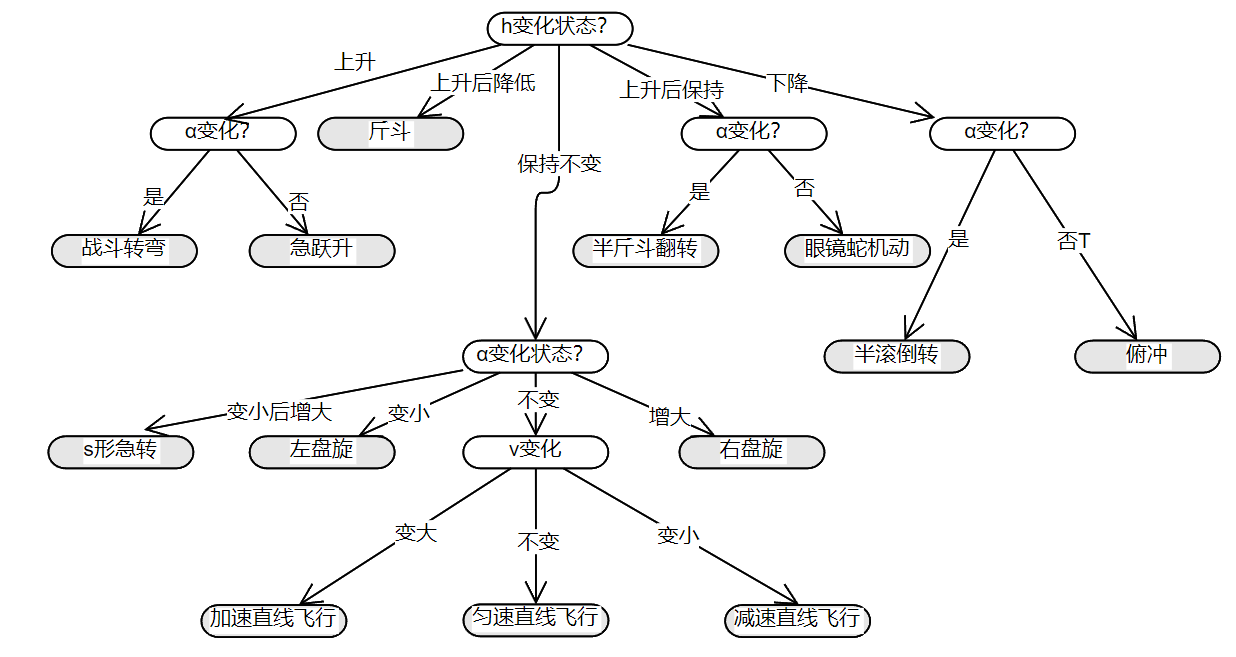
\includegraphics[width=\textwidth]{juece.png}
\caption{单个动作识别的决策树} % 标题
\label{five}
\end {figure}

上述识别过程即为动作描述量化模型。在完成单个动作的识别后,我们还需考虑时间间隔的划分策略,以及趋势的判别方式,我们将在下一部分进行建模分析。

\subsection{机动动作序列识别模型}

为了解决问题二,需要将附件数据进行清洗筛选,随后判断其变化趋势情况,就时间段输入到动作描述量化模型中,最后输出所有飞机的飞行动作序列。该序列包含每个unix时间对应下的飞机id与对应的动作。为此我们建立双窗口滑动趋势判断模型,根据变化趋势来识别时间序列片段的飞行参数变化情况与起止时间,随后利用问题一中提出的动作描述量化模型识别对应的动作。

\subsubsection{数据预处理过程}

分析观察数据,数据有个体丰富种类多样的特点。具体体现在一个文件代表一场战役,战役中含有敌我双方的若干飞机、导弹与干扰弹等。这些战场上的实体在任意时段出现或是消失。要进行动作序列的生成,需要将属于每个个体的条目分别划分出来。同时,每架飞机和每一枚导弹各自都归属于某个阵营,这一参数可以用于分析战场态势。同时,鉴于不同型号飞机的结构设计不同,对应的设计指标也就不同,需要就飞机的具体型号进行划分,以便决定后续各机型的参数。对于此类重要信息,我们选取一场战斗中数据进行分析总结,列出表(\ref{tp})。



\begin{table}[h]
\centering
\caption{战场上的重要个体信息统计}
% \begin{tabular}{|l|l|l|l|l|l|l|}
%     id & Type & Color & Coalition & Name & Group & Country \\ \hline
%     102 & Air+FixedWing & Red & Allies & E-2C & Red AWACS \#002 & xu \\ \hline
%     202 & Air+FixedWing & Blue & Enemies & E-2C & Blue AWACS \#001 & us \\ \hline
%     106 & Air+FixedWing & Red & Allies & J-11A & Red J-11A \#001 & xu \\ \hline
%     10A & Air+FixedWing & Blue & Enemies & Su-27 & Blue Su-27 \#001 & ru \\ \hline
%     109 & Air+FixedWing & Red & Allies & Su-33 & Red Su-33 \#001 & xu \\ \hline
%     107 & Air+FixedWing & Blue & Enemies & F-15C & Blue F-15C \#002 & us \\ \hline
%     108 & Air+FixedWing & Red & Allies & Su-33 & Red Su-33 \#002 & xu \\ \hline
%     10C & Air+FixedWing & Red & Allies & J-11A & Red J-11A \#005 & xu \\ \hline
%     105 & Air+FixedWing & Red & Allies & J-11A & Red J-11A \#002 & xu \\ \hline
%     10B & Air+FixedWing & Blue & Enemies & J-11A & Blue J-11A \#001 & cn \\ \hline
%     104 & Air+FixedWing & Blue & Enemies & J-11A & Blue J-11A \#002 & cn \\ \hline
%     10E & Air+FixedWing & Blue & Enemies & F-15C & Blue F-15C \#001 & us \\ \hline
%     10F & Air+FixedWing & Red & Allies & J-11A & Red J-11A \#003 & xu \\ \hline
%     110 & Air+FixedWing & Blue & Enemies & J-11A & Blue J-11A \#003 & cn \\ \hline
%     205 & Weapon+Missile & Red & Allies & R-27ET & <missing> & xu \\ \hline
%     204 & Weapon+Missile & Blue & Enemies & R-27ET & <missing> & cn \\ \hline
%     706 & Weapon+Missile & Red & Allies & R-27ER & <missing> & xu \\ \hline
%     707 & Weapon+Missile & Blue & Enemies & AIM-120B & <missing> & us \\ \hline
%     360B & Weapon+Missile & Blue & Enemies & R-27ER & <missing> & cn \\ \hline
%     12406 & Weapon+Missile & Red & Allies & R-77 & <missing> & xu \\ \hline
%     1250B & Weapon+Missile & Blue & Enemies & R-73 & <missing> & cn \\ \hline
%     110A & Weapon+Missile & Blue & Enemies & R-27ER & <missing> & ru \\ \hline
%     24F0C & Weapon+Missile & Red & Allies & R-73 & <missing> & xu \\ \hline
%     2BB04 & Weapon+Missile & Blue & Enemies & R-77 & <missing> & cn \\ \hline
%     4F0A & Weapon+Missile & Blue & Enemies & R-27ET & <missing> & ru \\ \hline
%     7E0A & Weapon+Missile & Blue & Enemies & R-73 & <missing> & ru \\ \hline
%     301BC02 & Weapon+Missile & Violet & Neutral & R-73 (AA-11) & <missing> & <missing> \\ \hline
% \end{tabular}
\begin{tabular}{|l|l|l|l|l|}
    \hline
        Color(阵营颜色) & Type(型号) & Name(飞机) & name(导弹) & Country \\ \hline
        Red & Air+FixedWing & E-2C & R-27ET & xu \\ 
        Blue & Weapon+Missile & J-11A & R-27ER & us \\ 
        Violet(中立) & Misc+Decoy+Chaff(箔条干扰弹) & Su-27 & AIM-120B & ru \\ 
        ~ & Misc+Decoy+Flare(耀斑干扰弹) & Su-33 & R-77 & cn \\ 
        ~ & Misc+Container & F-15C & R-73 & \\ 
        ~ & Misc+Shrapnel(伤片弹) &&&\\ \hline
    \end{tabular}
\label{tp}
  \end{table}

在划分各个个体的数据后,观察按照unix时间排列的数据序列,发现存在数据缺失的现象,这是由于不同参数的采样率存在差异。为了分析的统一性,对这些数据进行插值。比较了线性插值,常数填补,以及移动均值方法,考虑到线性插值易受噪声影响,常数填补方式难以确定填补数值,而采用移动均值方法较好的减弱了噪声,因此采用该方法填补了缺失数值。


在完成上述步骤后,随机选取一架飞机的时间序列并绘制,观察到高度$h$较为稳定,而飞行速度$v$等飞行参数会存在不停止的小幅波动,如图(\ref{bdt})。原因在于飞机正常飞行时高度一般保持不变,但是空中气流的存在使得飞机速度和航向角等会发生波动。

\begin{figure}[htbp]
    \centering  %居中
    \subfigure[飞行真空速$v$]{   %第一张子图
    \begin{minipage}{0.4\textwidth}%大小总和超过textwidth则自动换行
    \centering    %子图居中
    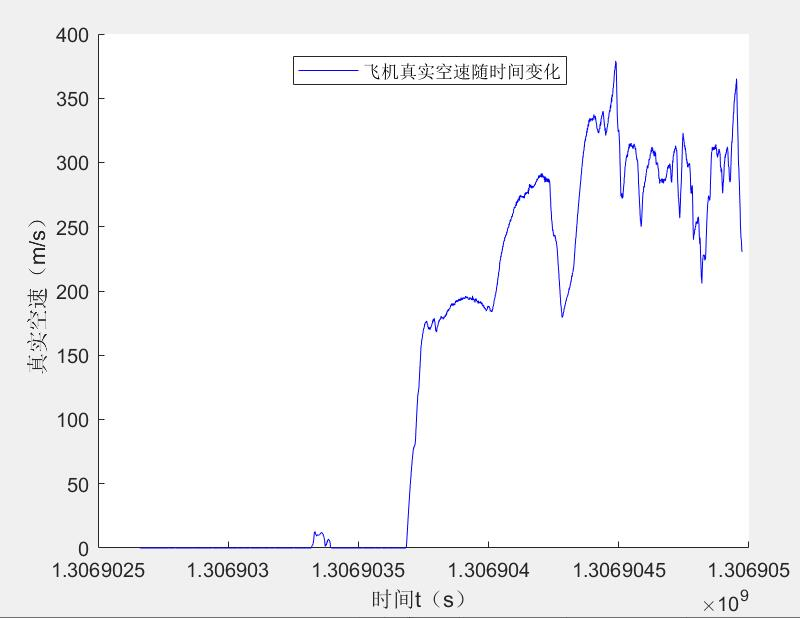
\includegraphics[width=\textwidth]{gdt.jpg}  %设置图片的输出大小倍数,这里是0.5倍大小输出
    \end{minipage}
    }
    \subfigure[飞行海拔高度$h$]{ %第二张子图
    \begin{minipage}{0.4\textwidth}
    \centering    %子图居中
    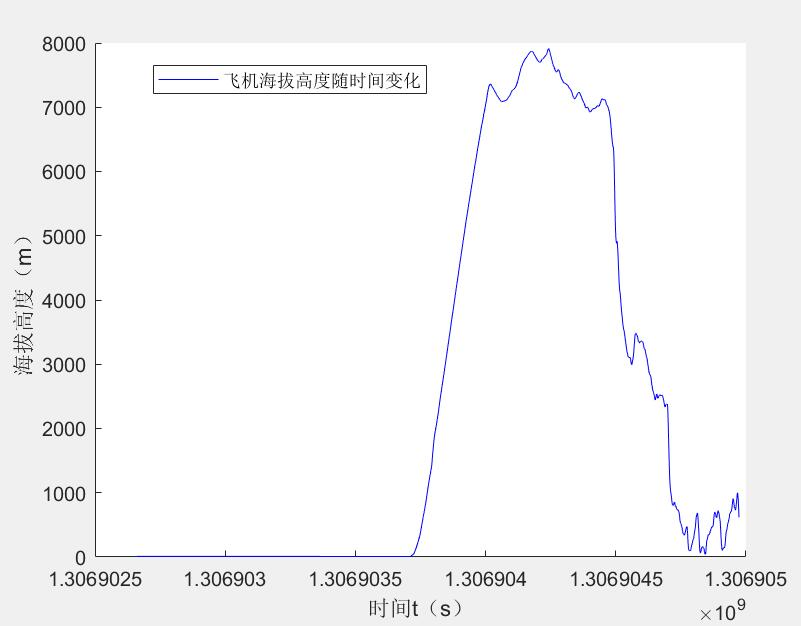
\includegraphics[width=\textwidth]{hbt.jpg}%以pic.jpg的0.5倍大小输出
    \end{minipage}
    }
    

    \caption{飞行参数同时间的变化关系图}    %大图名称
    \label{bdt}    %图片引用标记
\end{figure}
\newpage
针对航向角的变化问题,观察到航向角(偏航角)的数据处于$ 0\degree $-$ 360\degree $范围内,这是仪器本身结果所限。但是若要分析器变化趋势,直接使用该原始数据可能带来识别错误的现象。以右盘旋动作为例,在进行该动作时,偏航角变大,假设飞机开始转向时初始偏航角$\alpha_0=350\degree$,向右偏转$ 20\degree $,随后偏航角数据显示为$ 10\degree $。此时若用原始数据判断,则会判断出“先增后减再增”三段趋势,从而导致不能准确识别。为了解决这一问题,我们采用偏航角的累计变化量来代替原始数据,其基本思想是比较两相邻时刻的$ \Delta\alpha $值,若变化接近$ \pm 360\degree $,则直接取变化的累积量$ \alpha' $为下一时刻的偏航角值,计算方法由式\ref{phj}所列出。

\begin{equation}
    \alpha'_{t+1} = \begin{cases}
        \alpha'_{t} + \Delta \alpha+360\degree,&\Delta \alpha\to -360\degree \\
        \alpha'_{t} + \Delta \alpha-360\degree,&\Delta \alpha\to 360\degree \\
        \alpha'_{t} + \Delta \alpha,&else
    \end{cases}
    \label{phj}
\end{equation}

就处理前后的偏航角进行对比,得到下图(图\ref{hxj}):

\begin {figure}[h]
\centering % 居中显示
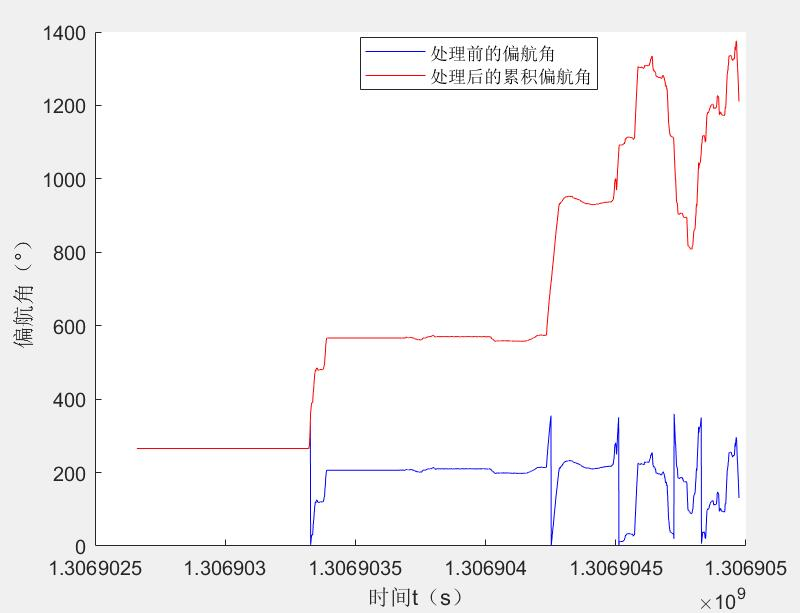
\includegraphics[width=0.6\textwidth]{phjt.jpg}
\caption{处理前原始航向角$\alpha$和处理后的$\alpha'$对比图} % 标题
\label{hxj}
\end {figure}

观察数据特点并对其做数据处理后,我们想要从参数序列中提取变化情况,即判断一段参数序列是平稳不变,还是上升或者下降。需要尽可能减少噪声带来的误判,并准确识别数据的变化趋势。我们尝试使用差分的方法,但是由于噪声的存在,无法正确识别可用信息。随后采用均值滤波后的序列进行差分,效果仍然不佳,且造成数据的突变特征被减弱。在上述尝试的基础上,我们又查阅相关资料\cite{9},提出了采用双滑动窗口的解决办法。

\subsubsection{序列趋势识别模型}

飞行各参数按照时间有序记录,因此飞行参数的五个维度$(h,\dot{h},\alpha,\dot{\alpha},v )$都可看作是一串序列,我们使用$\{x_1,x_2,x_3,...,x_m\}$代表时间标号,使用$\{y_1,y_2,y_3,...,y_m\}$代表第$i$个时刻下的飞行参数值。为了判断这串序列的趋势变化,采用最小二乘法计算其斜率,计算方法由式(\ref{er})给出。

\begin{equation}
    \left(\begin{array}{l}k \\b\end{array}\right)=\left(\boldsymbol{Y}^{\mathrm{T}} \boldsymbol{Y}\right)^{-1} \boldsymbol{Y}^{\mathrm{T}} \cdot \boldsymbol{X}
\label{er}
\end{equation}

所得k值由于是区间的变化趋势,较好的减弱了噪声的影响,我们根据k值来判断变化趋势。引入趋势变化基元,分为平直基元上升基元和下降基元三种,对应图(\ref{jiyuan})的三种情况。

\begin {figure}[h]
\centering % 居中显示
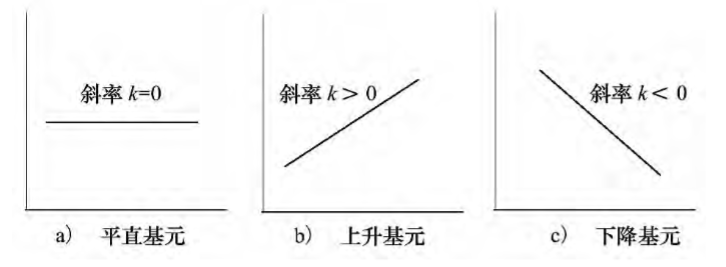
\includegraphics[width=0.8\textwidth]{jiyuan.png}
\caption{三种基元示意图} % 标题
\label{jiyuan}
\end {figure}

三种基元根据$k$的大小进行判断,设立$k_s$作为趋势阈值,当$k$大于$k_s$时识别为上升基元,小于$k_s$时识别为下降基元,当$-k_s<k<k_s$时判断是否满足高度变化阈值$\Delta_s$。趋势阈值$k_s$和高度变化阈值$\Delta_s$由我们所分析的数据的方差等统计量乘以系数得到,或是查阅相关资料得知。$k_s$的引入有效减少了错误检测平稳基元的情况。$\Delta_s$引入是为了判断长时间的机动变化,式(\ref{ds})满足,则序列趋势识别为上升或者下降。

\begin{equation}
|k\cdot m|>\Delta_s
\label{ds}
\end{equation}

综上所述,利用$k$值来识别基元种类的方法由图(\ref{jyz})所示。

\begin {figure}[h]
\centering % 居中显示
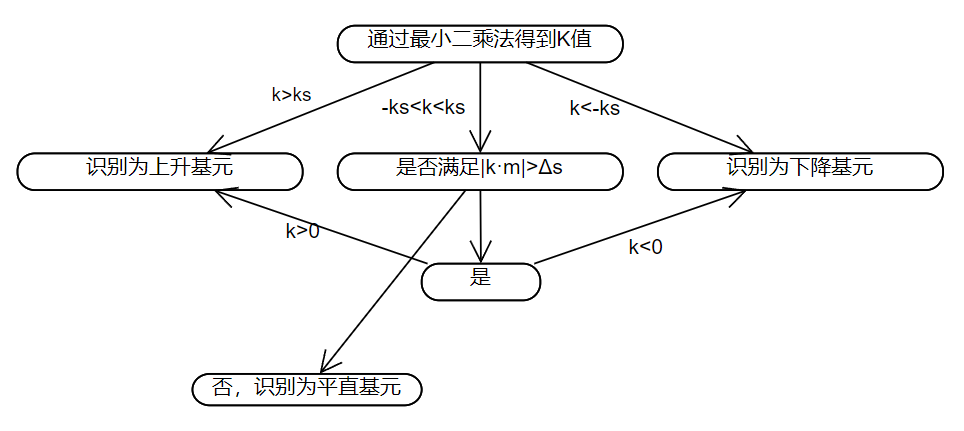
\includegraphics[width=\textwidth]{jiyuanz.png}
\caption{基元识别流程图} % 标题
\label{jyz}
\end {figure}

\subsubsection{双窗口趋势检测模型}
为了尽可能减少噪声影响的同时还可以检测趋势,使用双窗口滑动的方式来兼顾两个要求。构建一个滑动窗口和一个固定窗口,滑动窗口的大小保持不变,固定窗口的大小会发生变化。在初始状态下,滑动窗口和固定窗口的大小均为$m$,在算法执行过程中,滑动窗口向序列前方滑动来分析局部趋势$k_h$,固定窗口扩大相同长度来记录分析整体趋势$k_g$。窗口的行为由当前窗口分析出的基元结果来决定。

当窗口内的基元种类为上升或者下降时,此时滑动窗口向前移动一个单位,固定窗口相应扩大,再次考察移动后的$k_h$值,直至识别出基元的类型产生变化。当基元的类型产生变化时,根据$k_g$将固定窗口中的基元识别结果输出,作为该段的基元检测类型。同时将固定窗口的起始点位置移动置滑动窗口的起始点处,窗口大小重置为原长度$m$。

若窗口内的基元种类时平直状态时,滑动窗口向前移动一个单位,固定窗口同样扩大相同长度来记录分析整体趋势,此时需要考虑滑动窗口的$k_h$与固定窗口中的$k_g$之间的差值$\Delta k$,此时对应以下三种情况:

\begin{enumerate}
    \item $|k|>k_s$时将固定窗口中的数据识别为平直基元,并将固定窗口的数据识别为平直趋势,将固定窗口的长度重置,起点移动至滑动窗口的起点处。
    \item $|k|>k_s$且$\Delta k > \Delta s$则将固定窗口的行为识别为上升或下降,随后转至上一状态。
    \item $|k|>k_s$且$\Delta k < \Delta s$则继续向前滑动,扩大固定窗口的大小。
\end{enumerate}

综合上述过程,总结序列基元识别的状态转移图如图(\ref{slide})所示。

\begin {figure}[h]
\centering % 居中显示
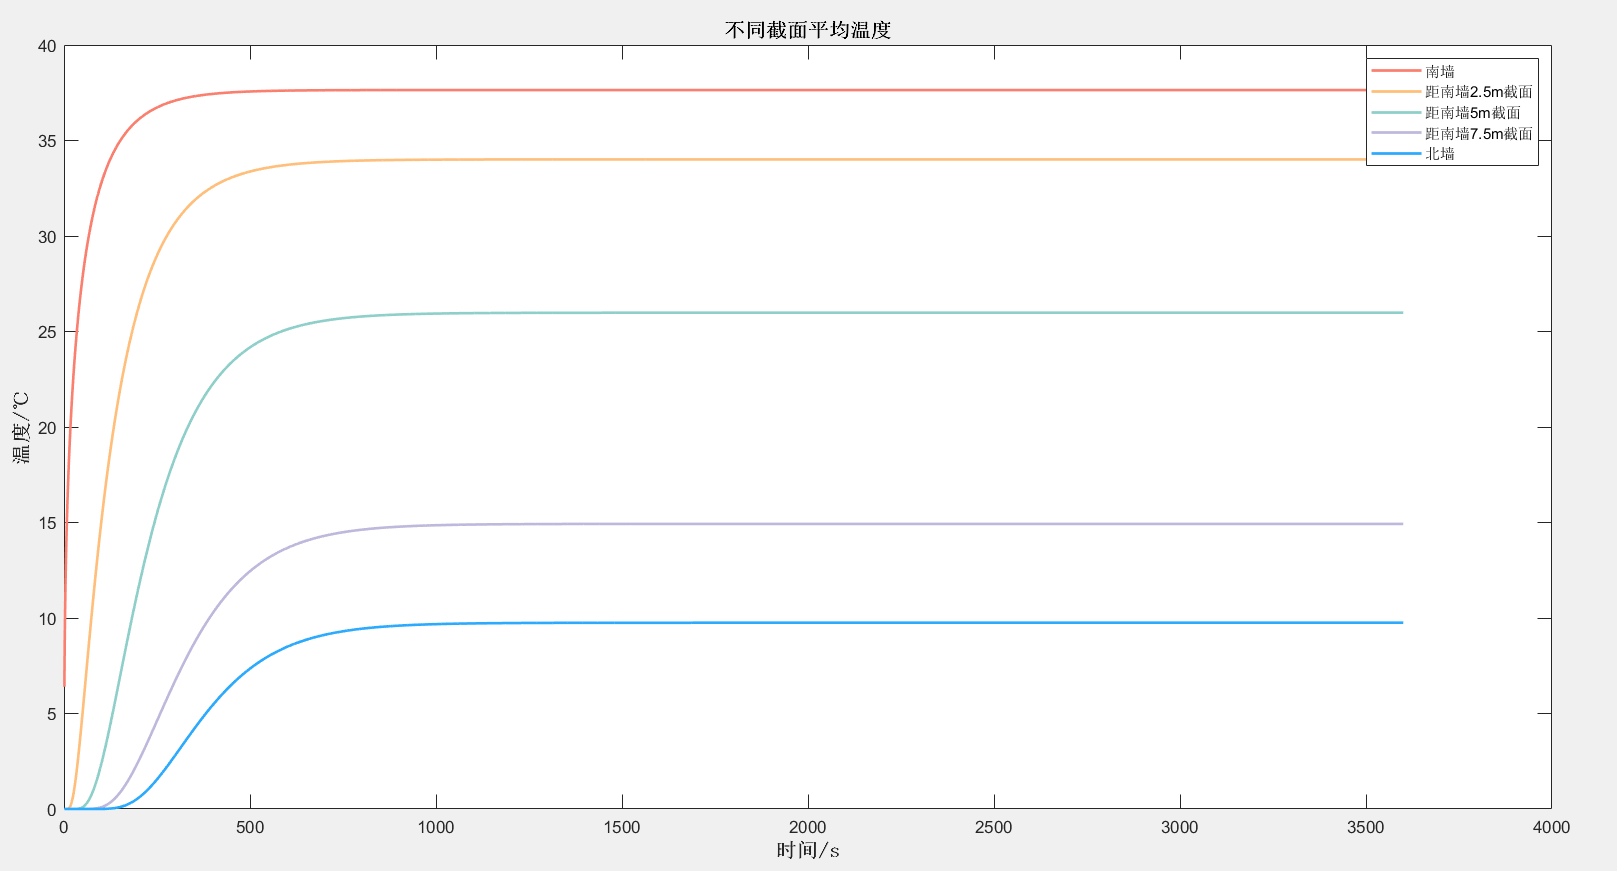
\includegraphics[width=\textwidth]{slide.png}
\caption{双滑窗移动状态转移图} % 标题
\label{slide}
\end {figure}

\newpage 
经过滑窗处理后,原始数据经过被分段处理,分段的标准是趋势的变化情况。我们根据基元的上升下降和平直三种趋势,将飞机参数划分为相应的变化段。我们认为在一个动作执行过程中,飞行参数变化情况为$A(h,\dot{h},\alpha,\dot{\alpha},v )$保持不变,故机动动作段如图(\ref{huafen})中划分的结果所示。
\begin {figure}[h]
\centering % 居中显示
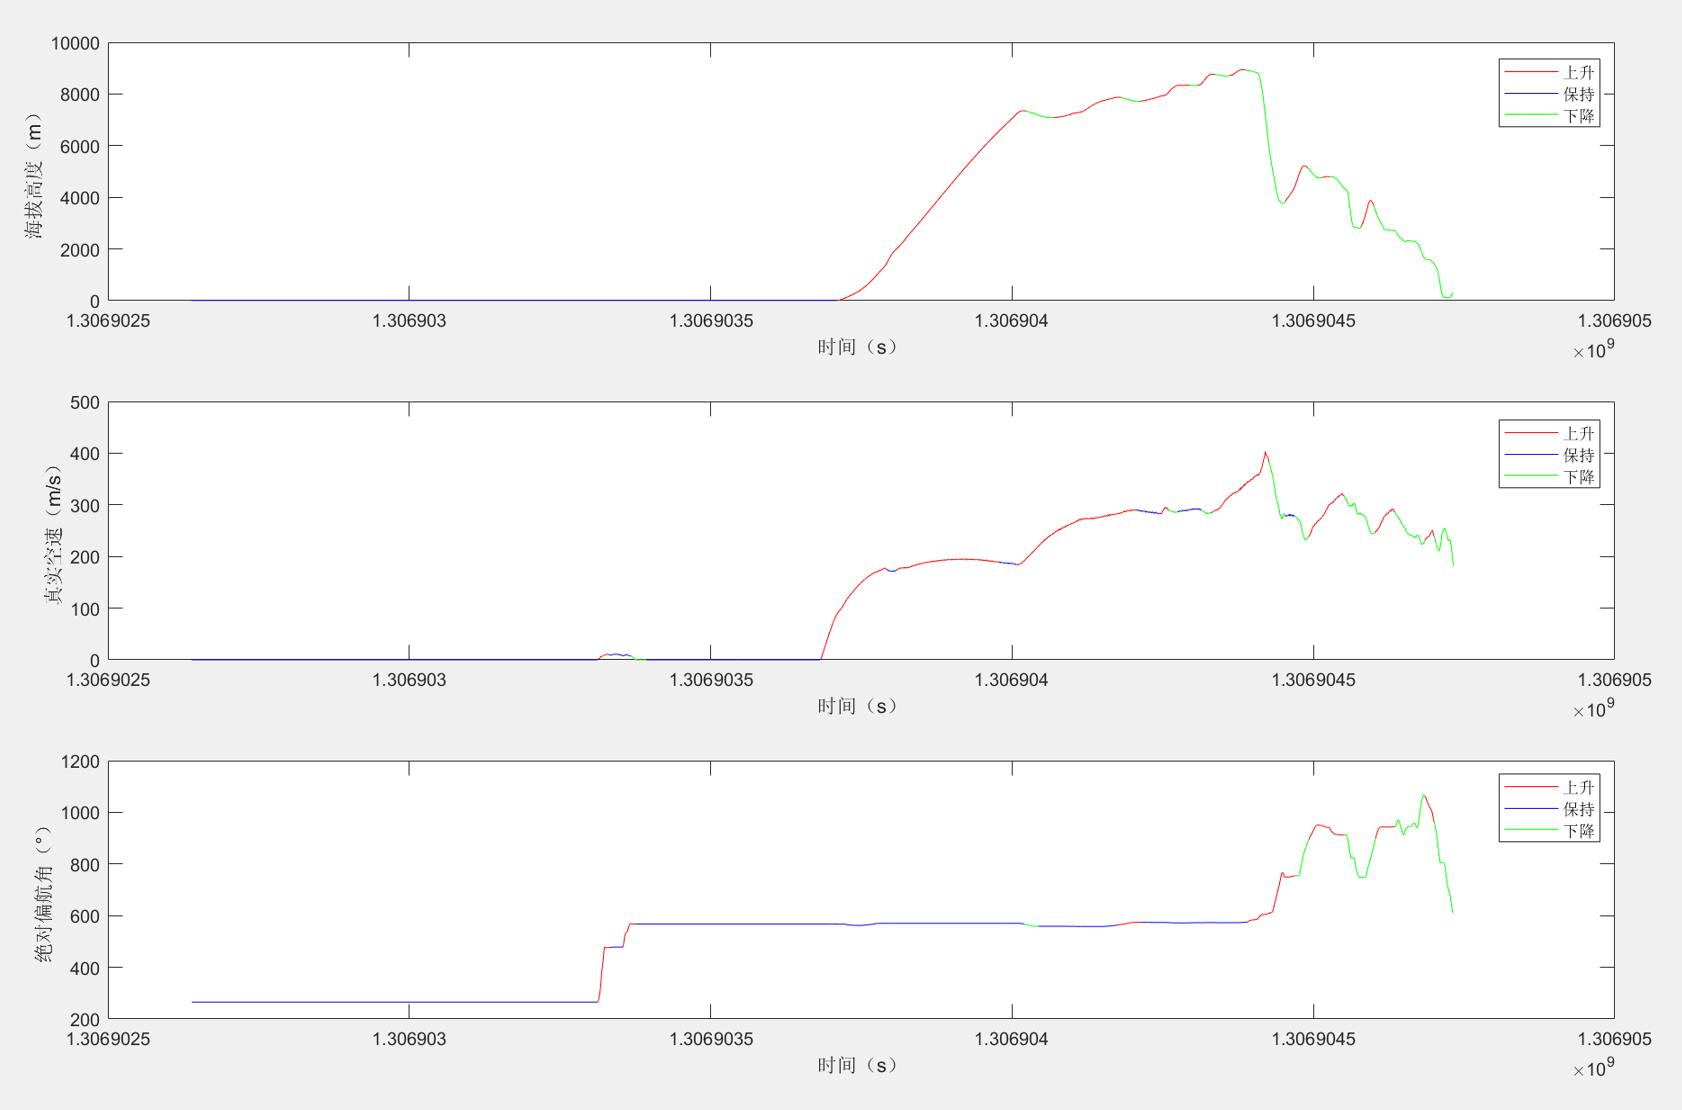
\includegraphics[width=0.85\textwidth]{d.jpg}
\caption{变化趋势划分结果(以$h,v,\alpha$为例)} % 标题
\label{huafen}
\end {figure}

以该图为例,取偏航角处上升的时间段分析,此时对应其余几个飞行参数的动作都是没有发生变化,对应到决策树的叶子节点为向右盘旋,其余推断过程以此类推。由于飞机操纵者习惯的差异和战场势态的变化,飞行动作执行时间可能不同。采用固定时间窗口进行动作划分,则很容易导致长动作被错误分割为多个更小动作。该方法可以很大程度上减少的这一错误划分现象。在得到动作段后,机动动作的种类可以由5.1中提出的决策树进行识别。



\subsubsection{飞机动作序列切割}

结合前文所述的飞机动作描述和量化模型,序列趋势识别模型以及双窗口趋势检测模型可以对一段飞机的飞行数据进行分析,得到每个时刻的动作序列结果。以表格形式展示以文件名为“51st Bisons vs CNF Rd 1”的前八架飞机的部分结果,如附件中表(\ref{dongzuo})所示。同时使用数字代表各个飞行动作,该文件中所有飞机的可视化结果如图(\ref{dzx})所示:

\begin {figure}[h]
\centering % 居中显示
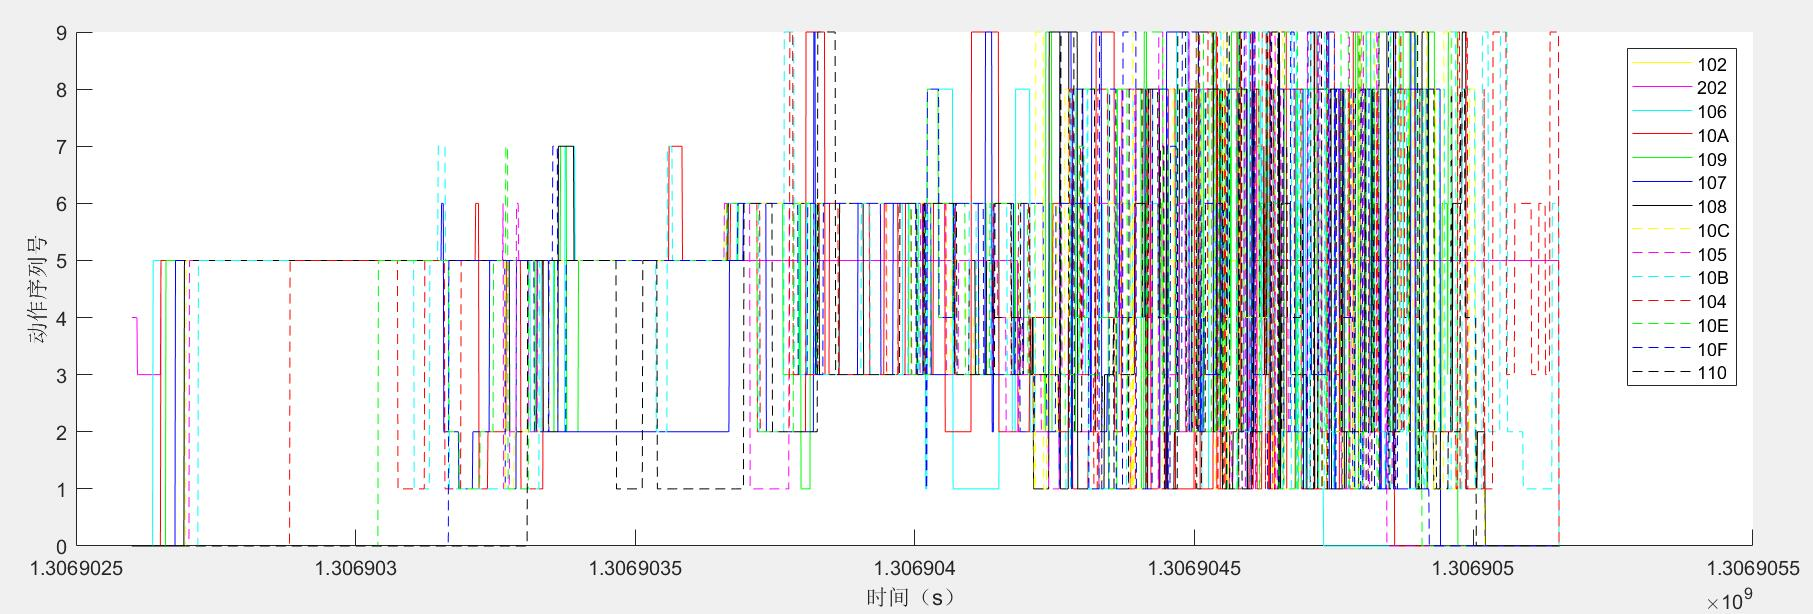
\includegraphics[width=\textwidth]{1zhuan.jpg}
说明:y轴上的数字对应各战斗动作。其中0:未出现;1:左盘旋;  2:右盘旋;  3:急跃升;  4:俯冲;  5:水平匀速直线; 6: 水平减速直线;7:水平加速直线;  8:半滚倒转; 9: 战斗转弯。
\caption{“51st Bisons vs CNF Rd 1”的动作序列} % 标题
\label{dzx}
\end {figure}

\subsection{子动作序列意图识别模型}
在这一部分,我们需要根据敌我双方之间的距离$d$与战备距离$d_s$的大小先划分为战斗意图和非战斗意图,在战斗意图中由根据战斗优势进行区分意图。下面分别介绍战机之间距离的计算方法,以及战斗优势的计算方法。

\subsubsection{敌我双方战机距离计算}

由附件材料可知,飞机记录的空间位置信息是由经纬度和高度$h$构成的,使用matlab中的geodetic2ned函数,将一架飞机的经纬度高度作为参考点,另一架飞机的相应参数输入后便可计算得出两架飞机之间的距离$d$.为了后续重要参数的确定,我们提取了原数据中的统计量(均值$ \mu_{d} $ 和方差$ \sigma_{d} $ ):每一架发射导弹的飞机距离其最近敌机的距离组成的统计值的均值和方差。

% 战备距离$d_s$是区分飞机意图的阈值,超过战备距离的飞机识别为非战斗意图巡航,而在战备距离中的飞机识别为战斗意图$y_i$,战斗意图集合$Y = \{$进攻,躲避$\}$。$d_s$

战备距离$d_s$是区分飞机意图的重要阈值,两军飞机在此阈值以外时,我们认为其没有处于战斗意图而是巡航意图。这里我们将非战斗意图,如侦察、巡逻、前往战场、返航全部认为是为“巡航”意图,只分析意图最重要、最复杂的“战斗意图”。因为每架飞机的战备距离$d_s$不同,所以这一重要阈值取自所有发射导弹的飞机同最近敌机之间距离$d$的统计量,即$\mu_d + 3\sigma$,该方法是通过大数定律来确定这一阈值,具有较高的可靠性。

分析战机数据,型号为“E-2C”的侦察机在空中稳定移动,几乎不参战,因此将其意图直接划归为“预警”。

\subsubsection{战斗优势计算}

考虑到战斗机在空中的机动动作,有时两架战机敌机没有适当的攻击角度即使距离很近也无法构成威胁。因此想要判断战机的作战意图,还需要结合战斗优势的评价来决定。该评价函数由角度,高度,距离和速度四个因素考虑,下面依次对这些因素进行分析。

\begin{enumerate}
    \item 角度因子评价函数$\Phi _{\theta}$
    
    战斗机发射导弹的过程,需要锁定目标在离轴角$\delta $的范围内,这样才能保证导弹在发射后能够制导到敌机位置。因此我们认为,敌机位于我方的离轴发射角$ \delta $内,则飞机所发射的导弹可以通过自动制导等方式攻击到敌机,而在$ \delta $之外的角度则超过越多,角度优势也就越小。综合以上分析,我们给出角度优势$ \Phi _{\theta}$的计算方法:

    \begin{equation}
        \large\Phi_{A}= \begin{cases}1, & 0 \leqslant \theta \leqslant  \delta \\ 1-\theta / 180\degree, & \text { 其他 }\end{cases}
    \end{equation}

    飞机与敌机的角度 $ \theta $ 在这里指飞机的空间角同飞机与敌机连线之间的夹角大小。敌机和我方飞机的相对位置示意如图(\ref{xiangdui})所示。

    \begin {figure}[h]
    \centering % 居中显示
    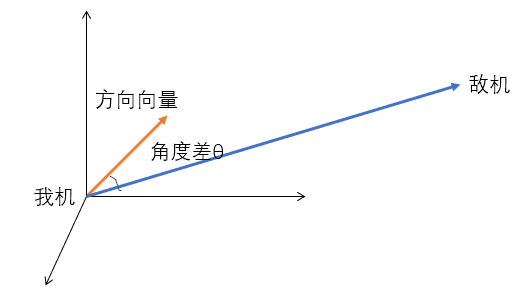
\includegraphics[width=0.6\textwidth]{weizhi.png}
    \caption{敌机和我机的相对位置关系} % 标题
    \label{xiangdui}
    \end {figure}

    根据附件数据中给出的偏航角 $ \alpha $ 和俯仰角 $ \beta $ 根据几何关系,可以给出该飞机在直角坐标系下的方向向量$ \vec{a}  $ :

    \begin{equation}
    \vec{a} = (cos\beta * sin \alpha,cos \beta * cos \alpha,sin\beta)
    \end{equation}

    又由两飞机之间的相对位置计算二者连线的方向向量$ \vec{b} $:

    \begin{equation}
    \vec{b} = (x_2,y_2,z_2)
    \end{equation}

    其中$ (0,0,0) $坐标原点处代表我方飞机,$ (x_2,y_2,z_2) $ 代表敌方飞机。

    计算两向量$ \vec{a} $和$ \vec{b} $的夹角可以计算飞机与敌机之间的角度$ \theta $:

    \begin{equation}
    \theta = arccos\frac{\vec{a}*\vec{b}}{|\vec{a}|*|\vec{b}|}
    \end{equation}

    ,这一$\theta$数值的统计量$\mu_{\theta}+\sigma{\theta}$便作为导弹的最大离轴发射角,这是因为飞机个体之间的差异,以及装配导弹的不同,一一确定离轴角并不现实,使用该统计量可以帮助得到合理的结果。
    \item 高度因子评价函数$\Phi _{h}$
    在两机作战过程冲,存在高度差$\Delta h$。处于较高位置的飞机可以将势能转化为动能,获得更大的能量优势与导弹的能量优势。但是在高度差过大的情况下,导弹需要进行大幅变向机动追踪,反而造成劣势。考虑上述原因,构造以下高度因子评价函数:

    \begin{equation}
        \large\Phi_{H}= \begin{cases}1, &  \Delta H_{\text {down }} \leqslant \Delta h \leqslant  \Delta H_{\text {up }} \\ \mathrm{e}^{-\frac{\Delta h - \Delta H_{\text {up }}}{\Delta H_{\text {up }}}}, & \Delta h> \Delta H_{\text {up }} \\ \frac{\Delta h- \Delta H_{\text {down }}}{\Delta H_{\text {down }}}, & \Delta h< \Delta H_{\text {down }}\end{cases}
    \end{equation}

    其中$ \Delta h _{down} $和$ \Delta h _{up} $分别代表保持最佳优势高度差的上下边界。该数据同样是利用原始数据中的我方发射导弹的战斗机同目标敌机之间的高度差统计量来确定,$\Delta h_{up} = \mu_h + \sigma_h$,$\Delta h_{down} = \mu_h - \sigma_h$

    
    \item 距离因子评价函数$\Phi _{d}$
    
    机载导弹存在不可逃逸距离\cite{10},在这一距离内,敌机无论以任何机动动作躲避,都无法避免被导弹击中。因此敌机处于不可逃逸区时其距离因子处于最大优势。为此,列出以下计算公式:

    \begin{equation}
        \large\Phi_{d}=\begin{cases}1,&L_{Mnear}\leq d \leq L_{Mfar}\\e^{\frac{L_{Mfar}-d}{L_{Mfar}}} &d>L_{Mfar}\\e^{\frac{d-L_{Mnear}}{L_{Mnear}}} &d<L_{Mnear}\end{cases}
        % \Phi_{d}=\begin{cases}1,&\Delta L_{Mnear}\leq d \leq \Delta L_{Mfar}\\e^{\frac{L_{Mfar}-d}{L_{Mfar}}} &d>\Delta L_{Mfar}\\e^{\frac{d-L_{Mnear}}{L_{Mnear}}} &d<\Delta L_{Mnear}\end{cases}
    \end{equation}
    
    其中$L_{Mnear},L_{Mfar}$为不可逃逸区的近边界和远边界。我们提取我方发射导弹的飞机同目标敌机之间的距离$d$,并依据大数定理将$L_{Mnear},L_{Mfar}$分别定为$\mu_d - \sigma_d,\mu_d + \sigma_d$

    \item 速度因子评价函数$\Phi _{v}$
    我方飞机飞行速度本身相较于目标应保持相对优势,以获得较高的速度能量,来应对不断变化的敌我态势和战场环境。当目标进入到我方导弹的不可逃逸区内,则此时我方飞机应维持与目标同样的飞行速度,当目标未进入到我方导弹的攻击区时,此时我方飞机应加大飞行速度以缩短敌我距离。我们依据这一作战策略,提出以下速度因子评价函数:

    \begin{equation}
        \large\Phi_v = \begin{cases}1,&L_{Mnear}\leq d \leq L_{Mfar}\\\mathrm{e}^{\left(V_{R }-V_{max}\right) / V_{B}},&d>L_{Mfar}\\\mathrm{e}^{\left(V_{\min }-V_{R}\right) / V_{B}},&d<L_{Mnear}\end{cases}
        % \Phi_v = \begin{cases}1,&\Delta L_{Mnear}\leq d \leq \Delta L_{Mfar}\\\mathrm{e}^{\left(V_{R }-V_{max}\right) / V_{B}},&d>\Delta L_{Mfar}\\\mathrm{e}^{\left(V_{\min }-V_{R}\right) / V_{B}},&d<\Delta L_{Mnear}\end{cases}
    \end{equation}

    在这里$V_{max}$与$V_{min}$都使用攻击时发射导弹飞机的最大和最小速度。
\end{enumerate}

在分析完成各个因素的计算方法后,我们依次赋权重 $ \eta $ 来计算总体评价函数,得到如下式子:

\begin{equation}
\Phi = \eta_{1}\Phi_{\theta}+\eta_{2}\Phi_{h}+\eta_{3}\Phi_{d}+\eta_{4}\Phi_{v}
\end{equation}

各个权重的分配按熵权法进行计算,下面介绍权重的计算步骤。我们记录一场战役的情况,就一架我方飞机发射导弹进行攻击时的评价序列$A(\Phi_{\theta},\Phi_{v},\Phi{h},\Phi_{d})_{m*4}$因素来计算其权重$ \eta $。

首先计算第$ i $个对象对于第$ j $个指标的权重大小:

\begin{equation}
p_{ij} = \frac{a_{ij}}{\sum_{i=1}^{n}a_{ij}}
\end{equation}

,随后计算各个指标的熵$e_j$:

\begin{equation}
    e_j = -1/ln(n) \sum_{i=1}^{n} p_{ij}*ln p_{ij}
\end{equation}

随后计算变异系数$g_j$和各个指标所占权重$ \eta $:

\begin{equation}
    g_j = 1-e_j
\end{equation}
\begin{equation}
    \eta_j = \frac{g_j}{\sum_{j=1}^{4}g_j}
\end{equation}

我们就“J-11A”这一系列飞机使用熵权法,计算出该类飞机的权重特征,如下表所示:

\begin{table}[ht]
\centering
\caption{熵权法权重确定结果}
\begin{tabular}{|l|l|l|l|}
    \hline
        \diagbox{优势函数}{熵权法中的对应参数} & $e$ & $g$ & $\eta$ \\ \hline
        $\Phi_\theta$ & 0.9908 & 0.0092 & 0.3963 \\ \hline
        $\Phi_H$ & 0.9926 & 0.0074 & 0.3179 \\ \hline
        $\Phi_b$ & 0.9968 & 0.0032 & 0.1397 \\ \hline
        $\Phi_v$ & 0.9966 & 0.0034 & 0.1461 \\ \hline
    \end{tabular}

\label{label}
  \end{table}

可见对于该型号的飞机而言,作战角度优势$ \Phi_\theta $与作战高度优势$\Phi_h$较为重要。
\subsubsection{动作序列与战斗意图识别}

通过分析我机和敌机之间的距离$d$和战斗优势$\Phi$,可以分析出任意时刻战机的作战意图得出以下计算式,分析步骤如图(\ref{pdjc})所示。
\begin{equation}
    y = \begin{cases}
        \text{巡航},& d>d_s\\
        \text{攻击},& d<d_s\quad and\quad \Phi_{\text{我机}}>\Phi_{\text{敌机}}\\
        \text{躲避},& d<d_s\quad and\quad \Phi_{\text{敌机}}>\Phi_{\text{我机}}\\
    \end{cases}
\end{equation}
,其中战斗距离$ d $由5.3.1中提出的方法,利用matlab中geodetic2ned函数计算,战备距离$ d_s $由统计得出,战斗优势利用5.3.2中四个因素的战斗优势公式$\Phi = \eta_{1}\Phi_{\theta}+\eta_{2}\Phi_{h}+\eta_{3}\Phi_{d}+\eta_{4}\Phi_{v}
$计算而出。

\begin {figure}[h]
\centering % 居中显示
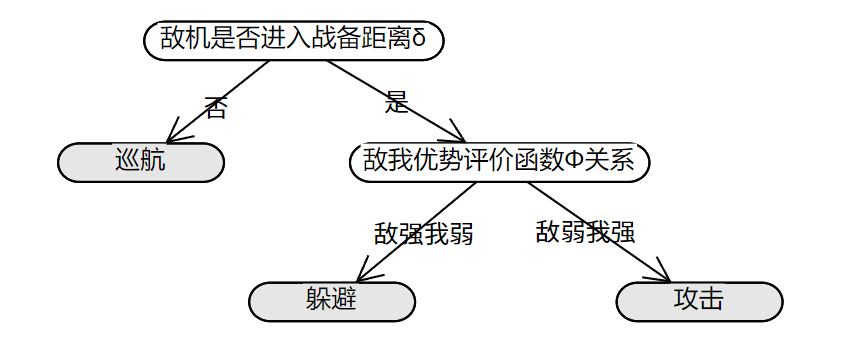
\includegraphics[width=0.8\textwidth]{yitu.png}
\caption{飞机意图判断决策图} % 标题
\label{pdjc}
\end {figure}


我们对整个战役中的意图进行识别,识别后对应到相应时段上的动作进行归类,将归属于同一意图$y_i$的动作序列$M\{m_1,m_2,...,m_n\}$归于同一集合。提取重复最多次的动作序列$M\in y_i$,认为该动作子序列对应意图为$y_i$。我们选取某架飞机在一场战斗中的动作序列和对应意图对应输出,并以意图变化时作为分割,输出以下图片:

\begin {figure}[h]
\centering % 居中显示
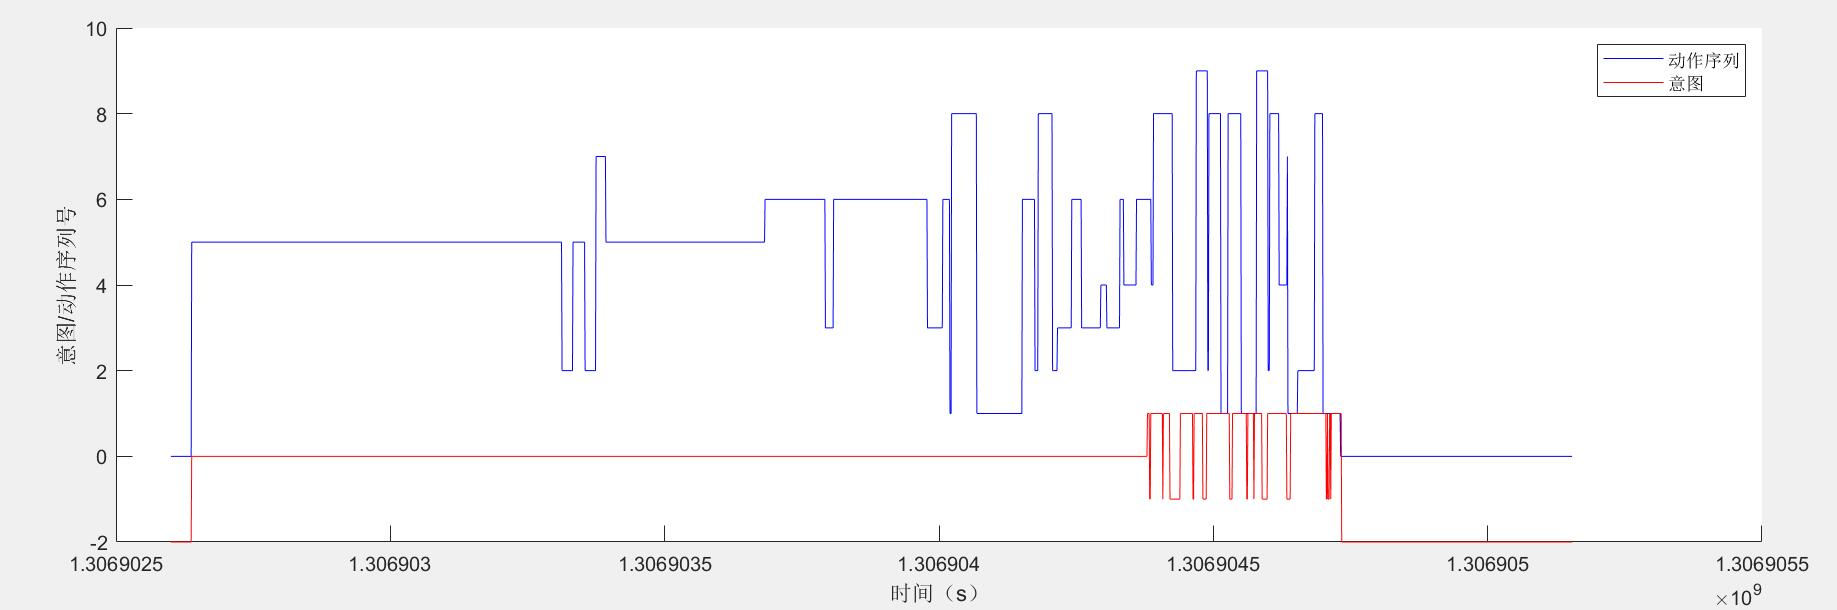
\includegraphics[width=\textwidth]{9.jpg}
说明:1代表攻击意图;0代表巡航意图;-1代表躲避意图。
\caption{动作序列和意图的对应关系图} % 标题
\label{five}
\end {figure}

\newpage
我们得到动作序列关于意图的划分后,进行动作的统计,得出以下结果:
\begin {figure}[h]
\centering % 居中显示
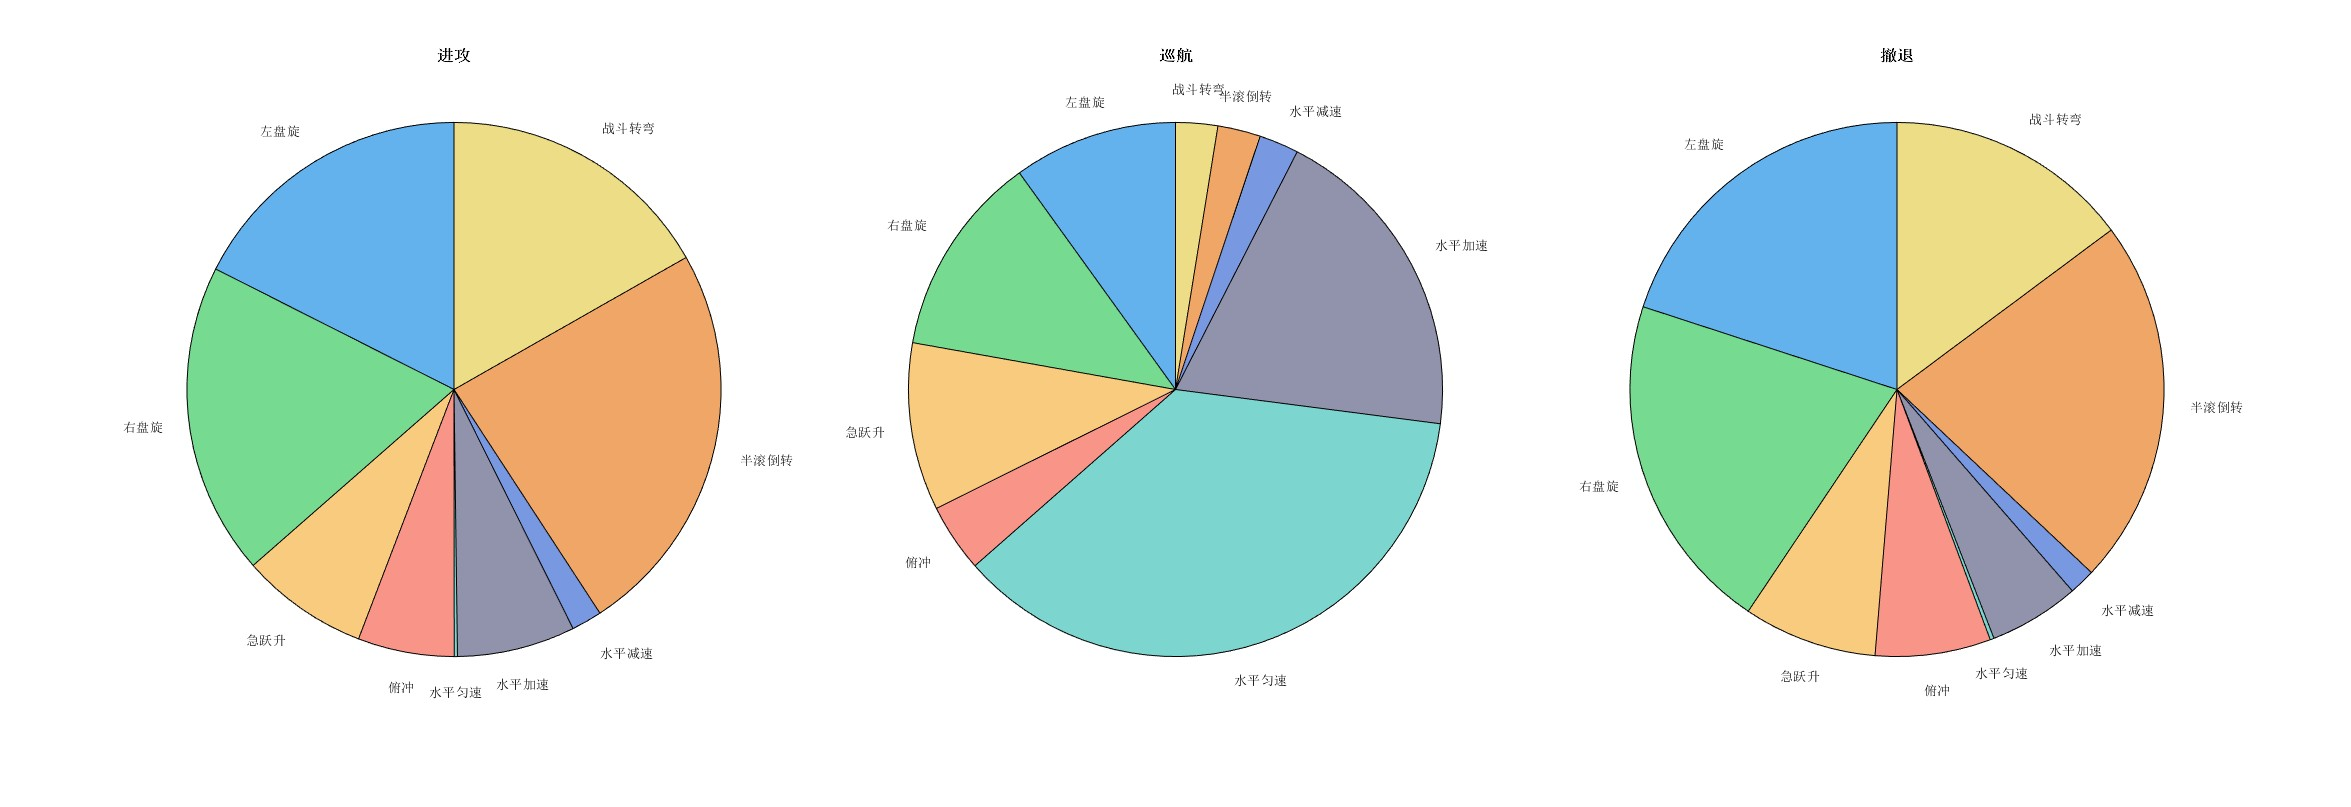
\includegraphics[width=\textwidth]{jieguo.jpg}
\caption{按意图划分的动作统计结果} % 标题
\label{five}
\end {figure}
由途中可知,处于巡航状态的战机由于受到的威胁较少,匀速直线飞行占了大部分;而处于进攻或是逃逸的飞机为了取得优势地位,通过较多转向,复杂机动等,变化航向角,高度等空间位置。可见基于意图的动作序列划分具有较好的解释性。

\subsection{整体态势识别判断模型}
我们通过分析,发现每场战斗双方都有预警机在场,介于预警机超长的作用范围,我们认为其不是影响态势的值得考虑的因素。同时,为了考虑势态的整体性,我们在第三问的基础上,从一个飞机的攻击优势拓展为一个联盟所有飞机的攻击优势,并且增加了干扰弹的影响。为了更直观的反应战场的势态情况,我们计算了战斗双方每一时刻获胜的概率值。

相关文献显示\cite{12},两种主要干扰弹“Misc+Decoy+Flare”和“Misc+Decoy+Chaff”的干扰效果为大约为70\%。干扰弹的存在会导致敌我双方发射导弹不能准确命中目标,最终导致占据优势的那一方作战效果大打折扣。在计算评估函数时由于是个体的意图判断,没有将干扰弹的因素考虑进去,而在整体态势识别过程中引入该因素。

为了判断战场形势,我们对场上战斗机的作战评价$\Phi$相加,并且加上干扰弹的判别因素,最终得到敌我双方战场的态势感知数值$f_B,f_R$。

\begin{equation}
f = \sum_{i \in B,R} \Phi_i
\end{equation}

若某一方占优势,如$f_R>f_B$,则在有干扰弹情况下对结果进行修正:

\begin{equation}
    f_R' = f_R - 0.7*(f_R-f_B)*q
\end{equation}

其中$q=\begin{cases}0,&\text{有干扰弹}\\1,&\text{无干扰弹}\end{cases}$,由修正后的敌我双方态势可以推知该场博弈中,哪方获胜的概率最大,计算公式如下。

\begin{equation}
    \text{红方:}P_R = \frac{f_R'}{f_R'+f_B} ,\text{蓝方:} P_B = \frac{f_B}{f_R'+f_B},\text{(假设红方占优)}
\end{equation}

我们在“51st vs 36th R1”这场战斗作为测试,计算了红蓝双方胜利的概率,最终整场战役的输出结果如图(\ref{p})所示:

\begin {figure}[h]
\centering % 居中显示
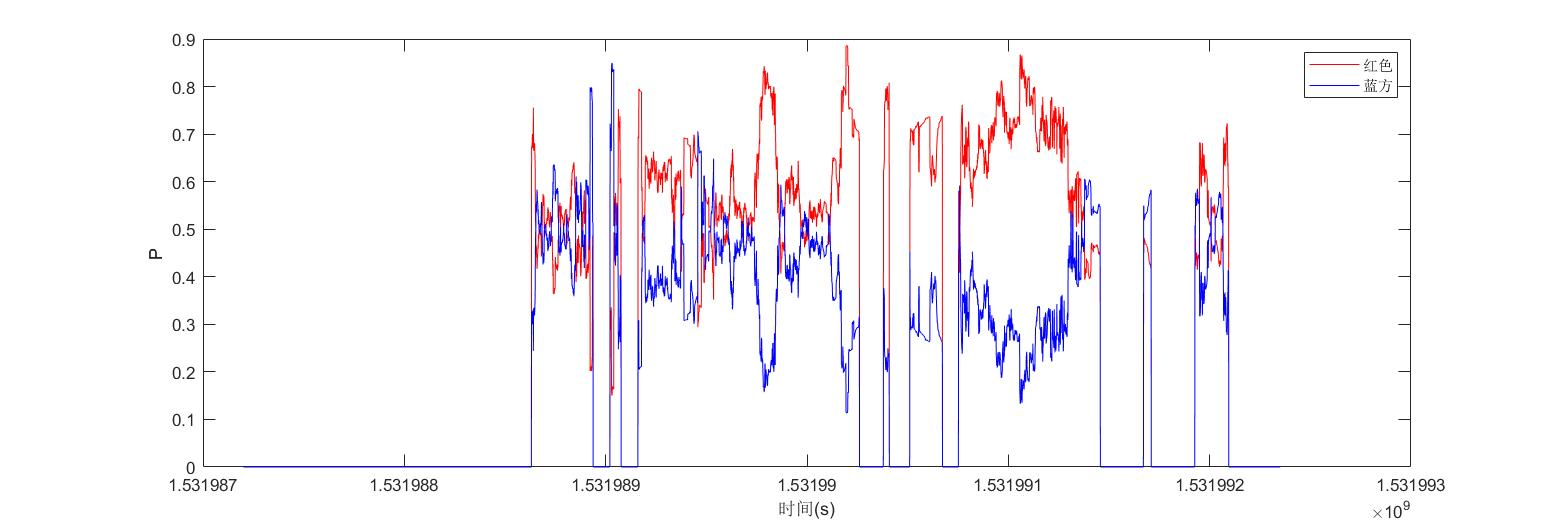
\includegraphics[width=\textwidth]{p.jpg}
\caption{51st vs 36th R1 战斗势态分析图} % 标题
\label{p}
\end {figure}

由图可知,在战斗开始时由于红蓝双方还未遭遇,双方并不存在所谓获胜概率一说,双方获胜概率均为0。双方遭遇之后,红蓝双方的获胜概率不断变化,反应双方战斗水平相当,战斗持续一段时间后都互相远离,结束战斗。


\section{七、模型的评价}


\subsection{模型的优点}
\begin{enumerate}
    \item 采用定性分析后的飞行参数确定飞行动作,提出飞行动作种类丰富,兼顾基本动作与特技动作。
    \item 采用双窗口法对变化的数据序列进行分析,有效减少了噪声影响,并且提取出数据的变化趋势。
    \item 使用时间作为桥梁联系飞机飞行意图和动作序列,有效利用了所给数据,并考虑统计意图和动作序列之间的关系,得出动作子序列和飞机意图之间的对应关系。
    \item 综合考虑了全局的战术意图情况,在势态感知中引入了干扰弹,有效利用了信息。
    \item 在确定阈值时,首先依据统计规律从原始数据中提取,在原始数据无法满足时,从参考文献中获得,如5.2.2中窗口大小依据飞机完成动作的最小时间确定,而趋势阈值$ k_s $的选取来自文献或是角度,速度差分的均值;5.3.1中的战备距离$d_s$由每架发射导弹的飞机同最近距离$d$的统计量:$3\sigma + \eta$;5.3.2中各项参数也有统计量所确定。
\end{enumerate}

\subsection{模型的缺点}
\begin{itemize}
    \item 对于多阶段的飞行动作识别还不够精确,仍然存在部分飞行参数趋势划分有误的情况。
    \item 飞行意图仅有数种,不能很好的覆盖复杂飞行战术。
\end{itemize}

\subsection{模型的推广与改进}

本模型许多重要参数均来源于数据的统计量,并且针对不同的飞机都做了单独的统计,因此具有较好的移植能力。若能给予更多关于导弹的信息,如俯仰角和偏航角等,我们可以建立更精确的模型。同时,可以应用基尼系数增益等指标优化决策树节点的生成情况,以此提高运算效率。
\newpage
\bibliographystyle{unsrt} %规定了参考文献的格式
\begin{center}
\bibliography{reference} %调出LaTeX生成参考文献列表
\end{center}

%----------- 附录 ----------
\newpage
\section{附件}
\textbf{附件清单:}
\begin{itemize}
    \item data-process-fun-1.m
    
    作用:分析导弹,获取在一场战斗中出现的所有导弹,以及初次出现的位置和同时刻最近敌机的位置使用统计的方法,计算出合理的战斗范围,从而在综合判断战术意图。

    \item action-main.m 
    
    作用:匹配相应的动作向量,找到对应的动作。

    \item action-choose.m 
    
    作用:使用欧式距离求出最接近的动作元类别

    \item jiyuan-mian.m
    
    作用:对实际数据进行动作向量基元分析,得到每时每刻的动作各维度动作基元

    \item TAS.m
    
    作用:获得单一维度的基元分析

    \item EWM.m
    
    作用:使用熵权法,正确的得到对应价值函数的权值

    \item qiucanshu.m
    
    作用:求取所有的价值函数的必要参数

    \item data-process-fun.m
    
    作用:最初的数据预处理,将固定翼飞机的各种信息整合提取出来

    \item main.m
    
    作用:意图分析主要代码

\end{itemize}

\textbf{data-process-fun-1.m}

\begin{lstlisting}[language=matlab]
    %%%%%%%%%%%%%%%%%%%%%%%%%%%%%%%%%%%%%%%%%%%%%%%%%%%%%%%%%%%%%%%%%%%%%%%%%%%
%数据预处理函数,保存矩阵文件
clc;clear;
%%%%%%%%%%%%%%%%%%%%%%%%%%%%%%%%%%%%%%%%%%%%%%%%%%%%%%%%%%%%%%%%%%%%%%%%%%%

%矩阵的第1列舍去,19,38,39列完全缺失,3,13:18是包含字符的标识
%name_mat id Type Color Coalition Name Group Country 包含不同飞机的基本信息矩阵
%data_mat 数据元胞数组,第一维代表飞机标号,第二维代表数据号,第三维代表数据类型
filename_mat = ["51st Bisons vs CNF Rd 1","51st Bisons vs CNF Rd 2","51st vs 36th R1","51st vs 36th R2","51st vs uvaf round 1","51st vs uvaf round 2","51st vs uvaf round 3","51stKIAP_vs_36th_Round_1","51stKIAP_vs_36th_Round_2","51stKIAP_vs_107th_Round_1"];

for num_now = 1:10
    filename = filename_mat(num_now);
    data = readmatrix(strcat('raw data\',filename,'.csv'), 'OutputType', 'string'); %以字符串格式读入数据
    mkdir(strcat('C:\Users\ASUS\Desktop\第一次国赛模拟\data\',filename));
    data_mat = {};
    name_mat = strings(0,0);
    num = 0; %目前导弹数
    for i = 1:height(data) %按照行读取
        data_now = data(i,:); %读取行  
        id = data_now(3);%此行id
        if isempty(name_mat)
            num = num + 1;
            name_mat(num,:) = [data_now(2),data_now(3),data_now(13),data_now(15),data_now(4:6)]; %录入新导弹信
            sel = 1;
        else
            [sel,loc] = ismember(id,name_mat(:,2),'row');
        end
        if ~sel %没有数据
            num = num + 1;
            name_mat(num,:) = [data_now(2),data_now(3),data_now(13),data_now(15),data_now(4:6)]; %录入新导弹信息
        end
    end
    %处理完毕,提取飞机信息
    Type = name_mat(:,3); %获取飞行物类别
    TF = contains(Type,'Weapon+Missile');
    index = find(TF==1); % 目标索引
    name_mat = name_mat(index,:); %修建名字矩阵
    Missile_mat = name_mat;
    save(strcat('C:\Users\ASUS\Desktop\第一次国赛模拟\data\',filename,'\Missile_data.mat'),"Missile_mat"); %保存名字矩阵
end

\end{lstlisting}

\textbf{action-main.m }
\begin{lstlisting}[language=matlab]
    %%%%%%%%%%%%%%%%%%%%%%%%%%%%%%%%%%%%%%%%%%%%%%%%%%%%%%%%%%%%%%%%%%%%%%%%%%%
%使用状态基元向量,将判别树转化为聚类中心确定的向量聚类
clear;clc;
%%%%%%%%%%%%%%%%%%%%%%%%%%%%%%%%%%%%%%%%%%%%%%%%%%%%%%%%%%%%%%%%%%%%%%%%%%%
action = strings(1,9);
action(1) = '左盘旋';
action(2) = '右盘旋';
action(3) = '急跃升';
action(4) = '俯冲';
action(5) = '水平匀速';
action(6) = '水平加速';
action(7) = '水平减速';
action(8) = '半滚倒转';
action(9) = '战斗转弯';
action_vec = [0,-1,0;0,1,0;1,0,-1;-1,0,1;0,0,0;0,0,1;0,0,-1;-1,1,1;-1,-1,1;1,1,-1;1,-1,-1]; %最后两个是叠加态判断
war_name = ["51st Bisons vs CNF Rd 1","51st Bisons vs CNF Rd 2","51st vs 36th R1","51st vs 36th R2","51st vs uvaf round 1","51st vs uvaf round 2","51st vs uvaf round 3","51stKIAP_vs_36th_Round_1","51stKIAP_vs_36th_Round_2","51stKIAP_vs_107th_Round_1"];
path_root = 'C:\Users\ASUS\Desktop\第一次国赛模拟\data\'; %文件根目录
ans_root = 'C:\Users\ASUS\Desktop\第一次国赛模拟\问题2结果number\';
% for war_num = 1:10
war_num = 10;
    load(strcat(path_root,war_name(war_num),'\plane_data.mat')); %导入飞机飞行信息  需要提取时间轴 
    load(strcat(path_root,war_name(war_num),'\plane_name_data.mat')) %导入飞机信息 飞机id在 1 
    load(strcat(path_root,war_name(war_num),'\action_cell.mat')) %导入飞机动作信息  时间 1 2 3 
    clear ANSWER answer
    ANSWER = strings(1,length(plane_data)+1);
    ANSWER(1) = 'Unix time';
    ANSWER(2:length(plane_data)+1) = plane_name_data(:,1)';
    xlswrite(strcat(ans_root,war_name(war_num),'动作序列','.xlsx'),ANSWER,'sheet1','A1'); %写入标题
    %找有飞机出现的时间段
    for i = 1:length(plane_data)
        plane = plane_data{i};
        if ~isempty(plane)
            MIN_MAX(i,1) = min(plane(:,1));
            MIN_MAX(i,2) = max(plane(:,1));
        else
            MIN_MAX(i,1) = 10000000000000;
            MIN_MAX(i,2) = 0;
        end
    end
    min_time = min(MIN_MAX(:,1));
    max_time = max(MIN_MAX(:,2));
    t = min_time:max_time; %获取最大时间轴, 写入到目标矩阵第一列 数据结果矩阵 和最终矩阵相差一行
%     xlswrite(strcat(ans_root,war_name(war_num),'.xlsx'),t','sheet1','A2'); %写入标题
    time_long = length(t); %所有飞机的时间长度都应该是这个长度
    answer = strings(time_long,length(plane_data));
    answer(:,:) = '未出现'; %初始化矩阵
    for l = 1:length(plane_data)
        plane_action = action_cell{l};
        if ~isempty(plane_action) %有动作
            for r = 1:height(plane_action)
                action_vector = plane_action(r,2:4); %获得需判断向量
                chose = choose(action_vector);
                t0 = plane_action(r,1);
                index = find(t==t0); %获取时间行
                answer(index,l) = chose; %写入矩阵
            end
        end
    end
    xx = [t',answer];
    save(strcat(ans_root,war_name(war_num),'动作序列','.mat'),'xx');
% end

\end{lstlisting}

\textbf{action-choose.m}
\begin{lstlisting}[language=matlab]
    function index = choose(vec)
    %判断最接近的向量
        action_vec = [0,-1,0;0,1,0;1,0,-1;-1,0,1;0,0,0;0,0,1;0,0,-1;-1,1,1;-1,-1,1;1,1,-1;1,-1,-1]; %最后两个是叠加态判断
        for i = 1:11
            dis(i) = ((vec(1)-action_vec(i,1))^2+(vec(2)-action_vec(i,2))^2+(vec(3)-action_vec(i,3))^2)^0.5;%计算距离
        end
        [~,index] = min(dis);
        if index == 9
            index = 8;
        elseif index == 10 || index == 11
            index = 9;
        end
    end
\end{lstlisting}

\textbf{jiyuan-mian.m}
\begin{lstlisting}[language=matlab]
    %%%%%%%%%%%%%%%%%%%%%%%%%%%%%%%%%%%%%%%%%%%%%%%%%%%%%%%%%%%%%%%%%%%%%%%%%%%
clc;clear;
%使用基元分析,求出各个时间点的动作向量
%%%%%%%%%%%%%%%%%%%%%%%%%%%%%%%%%%%%%%%%%%%%%%%%%%%%%%%%%%%%%%%%%%%%%%%%%%%
%ALT 分析飞机海拔高度
%YAW 分析飞机航向角
%TAS 分析飞机空速
%上述函数使用滑窗法结合一维线性拟合得到基元分析结果
%dYAW 分析飞机航向角的变化率,有突变状态
%dALT 分析飞机海拔高度的变化率

%排列顺序按照 ALT dALT YAW dYAW TAS 
%输出,在对应战斗的文件夹下,输出action矩阵文件 

filename_str = ["51st Bisons vs CNF Rd 1","51st Bisons vs CNF Rd 2","51st vs 36th R1","51st vs 36th R2","51st vs uvaf round 1","51st vs uvaf round 2","51st vs uvaf round 3","51stKIAP_vs_36th_Round_1","51stKIAP_vs_36th_Round_2","51stKIAP_vs_107th_Round_1"];

for num_now = 1:10 %按照战斗场次遍历
    war_name = filename_str(num_now); %获取待处理的战斗名称
    
    path = strcat('C:\Users\ASUS\Desktop\第一次国赛模拟\data\',war_name,'\data_mat.mat');
    load(path); %导入data_mat2 
    plane_num = length(data_mat2); %获取战机架数
    for plane = 1:plane_num %按照一场战斗中的战机遍历
        data = data_mat2{plane};
        if ~isempty(data)
            alt = ALT(data)'; %获得高度基元            
            yaw = YAW(data)'; %获得航向角基元
            tas = TAS(data)'; %获得空速基元
            t = data(:,1); %获得时间序列  
            action_mat = [t(1:length(t)-2),alt,yaw,tas]; %组合为动作矩阵
            action_cell{plane} = action_mat;
        else
            action_cell{plane} = [];
        end
    end
   save(strcat('C:\Users\ASUS\Desktop\第一次国赛模拟\data\',war_name,'\action_cell.mat'),'action_cell');
end

\end{lstlisting}

\textbf{TAS.m}
\begin{lstlisting}[language=matlab]
    %%%%%%%%%%%%%%%%%%%%%%%%%%%%%%%%%%%%%%%%%%%%%%%%%%%%%%%%%%%%%%%%%%%%%%%%%%%
%滑窗线性检测
%处理空速
%%%%%%%%%%%%%%%%%%%%%%%%%%%%%%%%%%%%%%%%%%%%%%%%%%%%%%%%%%%%%%%%%%%%%%%%%%%
function type_mat1 = TAS(data)
%%%%%%%%%%%%%%%%%%%%%%%%%%%%%%%%%%%%%%%%%%%%%%%%%%%%%%%%%%%%%%%%%%%%%%%%%%%
    %关键参数
    w = 10;
    
%%%%%%%%%%%%%%%%%%%%%%%%%%%%%%%%%%%%%%%%%%%%%%%%%%%%%%%%%%%%%%%%%%%%%%%%%%%    
    velocity = data(:,11); %获得空速序列
    dvelocity = abs(diff(velocity));
    k_s = mean(dvelocity);
    delta_s = mean(dvelocity) * w;
    t = data(:,1); %获得时间序列  
    big_win_start = 1; %大小滑窗初始化
    big_win_end = 1+w;
    small_win_start = 1;
    small_win_end = 1+w;
    MAX_time_index = length(t);%序列长度
    index = 1;
    %1:上升 0:平稳 -1:下降 
    while small_win_end <= MAX_time_index %不断滑动检测小窗
        [p,~,~] = polyfit(t(small_win_start:small_win_end),velocity(small_win_start:small_win_end),1); %拟合小窗数据
        if small_win_start == big_win_start %初始化滑动窗
            if p(1) >= k_s
                Type = 1;
            elseif p(1) <= -k_s
                Type = -1;
            else
                Type = 0;
            end
            small_win_start = small_win_start + 1;
            small_win_end = small_win_end + 1;
            big_win_end = small_win_end;
        else
            if Type == 1
                if p(1) > 0 %前一刻和此刻都是上升
                    small_win_start = small_win_start + 1;
                    small_win_end = small_win_end + 1;
                    big_win_end = small_win_end;            
                else  %变号了,固定更新
                    type_mat(index) = 1;
                    index_mat(index) = big_win_end-1;
                    index = index + 1;
                    small_win_start = small_win_end;
                    small_win_end = small_win_start + w;
                    big_win_start = small_win_start;
                    big_win_end = small_win_end;
                    delta = 0;
                end
            elseif Type == -1
                if p(1) < 0 %前一刻和此刻都是下降
                    small_win_start = small_win_start + 1;
                    small_win_end = small_win_end + 1;
                    big_win_end = small_win_end;            
                else  %变号了,固定更新
                    type_mat(index) = -1;
                    index_mat(index) = big_win_end-1;
                    index = index + 1;
                    small_win_start = small_win_end;
                    small_win_end = small_win_start + w;
                    big_win_start = small_win_start;
                    big_win_end = small_win_end;
                    delta = 0;
                end
            else
                if abs(p(1)) >= k_s 
                    type_mat(index) = 0;
                    index_mat(index) = big_win_end-1;
                    index = index + 1;
                    small_win_start = small_win_end;
                    small_win_end = small_win_start + w;
                    big_win_start = small_win_start;
                    big_win_end = small_win_end;
                    delta = 0;            
                else 
                    delta = max(velocity(big_win_start:big_win_end))-min(velocity(big_win_start:big_win_end));
                    if abs(delta) >= delta_s
                        if delta > 0
                            type_mat(index) = 1;
                            index_mat(index) = big_win_end-1;
                            index = index + 1;
                            small_win_start = small_win_end;
                            small_win_end = small_win_start + w;
                            big_win_start = small_win_start;
                            big_win_end = small_win_end;
                            delta = 0;   
                        else
                            type_mat(index) = -1;
                            index_mat(index) = big_win_end-1;
                            index = index + 1;
                            small_win_start = small_win_end;
                            small_win_end = small_win_start + w;
                            big_win_start = small_win_start;
                            big_win_end = small_win_end;
                            delta = 0;
                        end
                    else
                        small_win_start = small_win_start + 1;
                        small_win_end = small_win_end + 1;
                        big_win_end = small_win_end; 
                    end
                end
            end
        end
    end
        
    type_mat(index) = Type; %保存最后一个状态
    index_mat(index) = MAX_time_index-2;
    type_mat1 = zeros('like',type_mat);
    type = type_mat(1);
    if type == 1
        type_mat1(1:index_mat(1)) = 1;
    elseif type == 0
        type_mat1(1:index_mat(1)) = 0;
    else
        type_mat1(1:index_mat(1)) = -1;
    end
    for l = 2:length(type_mat)
        type = type_mat(l);
        if type == 1
            type_mat1(index_mat(l-1):index_mat(l)) = 1;
        elseif type == 0
            type_mat1(index_mat(l-1):index_mat(l)) = 0;
        else
            type_mat1(index_mat(l-1):index_mat(l)) = -1;
        end
    end
    type_mat1 = type_mat1(1:MAX_time_index-2);
end

\end{lstlisting}
\textbf{EWM.m}
\begin{lstlisting}[language=matlab]
    %%%%%%%%%%%%%%%%%%%%%%%%%%%%%%%%%%%%%%%%%%%%%%%%%%%%%%%%%%%%%%%%%%%%%%%%%%%
clear;clc;
%使用熵权法求解权值
%相关函数 fun1 fun2 fun3 fun4
%%%%%%%%%%%%%%%%%%%%%%%%%%%%%%%%%%%%%%%%%%%%%%%%%%%%%%%%%%%%%%%%%%%%%%%%%%%
path_root = 'C:\Users\ASUS\Desktop\第一次国赛模拟\plane\';
load(strcat(path_root,'\plane_name_str.mat'));
load(strcat(path_root,'\plane_type_cell.mat'));
for n = 1:7 %研究战机型号
    sample = plane_type_cell{n};
    mat = zeros(height(sample),4); %样本结果矩阵
    for i = 1:height(plane_type_cell{n})
        dis = (sample(i,1)^2+sample(i,2)^2+sample(i,3)^2)^0.5;
        mat(i,:) = [fun1(sample(i,9),n),fun2(-sample(i,3),n),fun3(dis,n),fun4(dis,sample(i,10),sample(i,11),n)];
    end
    %使用mat矩阵求四个权值
    N = height(sample);
    p = zeros(N,4);
    for j = 1:4
        for i = 1:N
            p(i,j) = mat(i,j)/sum(mat(:,j));
        end
        E(j) = (-1/log(N)) *sum(p(:,j).*log(p(:,j))); %求出各个指标的熵 
    end
    g = 1-E; %计算变异系数
    for j = 1:4
        ita(j) = g(j)/sum(g);
    end
    answer(n,:) = ita; 
end
save('EWM.mat','answer');

\end{lstlisting}

\textbf{qiucanshu.m}
\begin{lstlisting}[language=matlab]
    %%%%%%%%%%%%%%%%%%%%%%%%%%%%%%%%%%%%%%%%%%%%%%%%%%%%%%%%%%%%%%%%%%%%%%%%%%%
clc;clear;
%逐个飞机分析 
%%%%%%%%%%%%%%%%%%%%%%%%%%%%%%%%%%%%%%%%%%%%%%%%%%%%%%%%%%%%%%%%%%%%%%%%%%%

path_root = 'C:\Users\ASUS\Desktop\第一次国赛模拟\plane\';
load(strcat(path_root,'\plane_name_str.mat'));
load(strcat(path_root,'\plane_type_cell.mat'));
canshu = zeros(7,7); %建立参数表 theta delta_H_down delta_H_up L_M_near L_M_far V_min V_max

index = 1;
for i = 1:7
    plane = plane_type_cell{i};
    theta = mean(plane(:,9))+std(plane(:,9));
    delta_H_down = -mean(plane(:,3)) - std(plane(:,3));
    delta_H_up = -mean(plane(:,3)) + std(plane(:,3));
    dis = (plane(:,1).^2+plane(:,2).^2+plane(:,3).^2).^0.5;
    L_M_near = mean(dis)-std(dis);
    L_M_far = mean(dis) + std(dis);
    a(i) = mean(dis) + 3*std(dis);
    V_min = min(plane(:,10));
    V_max = max(plane(:,10));
    canshu(index,:) = [theta,delta_H_down,delta_H_up,L_M_near,L_M_far,V_min,V_max];
    index = index + 1;
end
save('canshu.mat','canshu');

\end{lstlisting}

\textbf{data-process-fun.m}
\begin{lstlisting}[language=matlab]
    %%%%%%%%%%%%%%%%%%%%%%%%%%%%%%%%%%%%%%%%%%%%%%%%%%%%%%%%%%%%%%%%%%%%%%%%%%%
%数据预处理函数,保存矩阵文件
clc;clear;
%%%%%%%%%%%%%%%%%%%%%%%%%%%%%%%%%%%%%%%%%%%%%%%%%%%%%%%%%%%%%%%%%%%%%%%%%%%

%矩阵的第1列舍去,19,38,39列完全缺失,3,13:18是包含字符的标识
%name_mat id Type Color Coalition Name Group Country 包含不同飞机的基本信息矩阵
%data_mat 数据元胞数组,第一维代表飞机标号,第二维代表数据号,第三维代表数据类型
filename_mat = ["51st Bisons vs CNF Rd 1","51st Bisons vs CNF Rd 2","51st vs 36th R1","51st vs 36th R2","51st vs uvaf round 1","51st vs uvaf round 2","51st vs uvaf round 3","51stKIAP_vs_36th_Round_1","51stKIAP_vs_36th_Round_2","51stKIAP_vs_107th_Round_1"];

for num_now = 1:10
    clear ans d data data_mat data_mat2 data_now h i id index l loc name_mat now num plane_data sel TF TF1 Type
    filename = filename_mat(num_now);
    data = readmatrix(strcat('raw data\',filename,'.csv'), 'OutputType', 'string'); %以字符串格式读入数据
    mkdir(strcat('C:\Users\ASUS\Desktop\第一次国赛模拟\data\',filename));
    data_mat = {};
    name_mat = strings(0,0);
    num = 0; %目前飞机数
    for i = 1:height(data) %按照行读取
        data_now = data(i,:); %读取行  
        id = data_now(3);%此行id
        if isempty(name_mat)
            num = num + 1;
            name_mat(num,:) = [data_now(3),data_now(13:18)]; %录入新飞机信息
            loc = num;
            data_mat{loc} = []; %创建新飞机的时间状态矩阵
            sel = 1;
        else
            [sel,loc] = ismember(id,name_mat(:,1),'row');
        end
        if ~sel %没有数据
            num = num + 1;
            name_mat(num,:) = [data_now(3),data_now(13:18)]; %录入新飞机信息
            loc = num;
            data_mat{loc} = []; %创建新飞机的时间状态矩阵
        end
        plane_data = data_mat{loc}; %获取到指定飞机的时间矩阵
        h = height(plane_data);
        plane_data(h+1,:) = [data_now(2),data_now(4:12),data_now(20:37),data_now(40:43)];
        data_mat{loc} = plane_data;
    end
    %处理完毕,提取飞机信息
    Type = name_mat(:,2); %获取飞行物类别
    TF = contains(Type,'Air+FixedWing');
    index = find(TF==1); % 目标索引
    name_mat = name_mat(index,:); %修建名字矩阵
    plane_name_data = name_mat;
    save(strcat('C:\Users\ASUS\Desktop\第一次国赛模拟\data\',filename,'\plane_name_data.mat'),"plane_name_data"); %保存名字矩阵
    %开始插值
    ll = 1;
    for i = 1:length(index) %遍历飞机
        d = data_mat{index(i)};
        if height(d) >= 10 %数据太少,不用,可能会导致数据缺失
            for l = 1:width(d) %遍历数据列
                now = d(:,l);
                TF1=ismissing(now);% 查找缺失值,TF是逻辑矩阵 
                delta = length(now) - length(TF1);
                TF = TF1;
                % 填充缺失值
                if delta >= 5
                    while max(TF) % 如果还存在缺失值就继续插补
                        now = fillmissing(now,'movmean',5); % 使用窗口长度为 5 的移动均值替换数据中的 NaN 值 
                        TF=ismissing(now);% 查找数据中的缺失值,TF是逻辑矩阵,利用TF可以找到now内的缺失值
                    end
                    d(:,l) = now;
                end
            end
            data_mat2{i} = d;
        else
            warn(ll) = i;
            ll = ll + 1;
            warning('Data is too small!');
            save(strcat('C:\Users\ASUS\Desktop\第一次国赛模拟\data\',filename,'\warn.mat'),'warn');
        end
    end 
    plane_data = data_mat2;
    save(strcat('C:\Users\ASUS\Desktop\第一次国赛模拟\data\',filename,'\plane_data.mat'),'plane_data');
end

\end{lstlisting}

\textbf{main.m}
\begin{lstlisting}[language=matlab]
    %%%%%%%%%%%%%%%%%%%%%%%%%%%%%%%%%%%%%%%%%%%%%%%%%%%%%%%%%%%%%%%%%%%%%%%%%%%
clear;clc;
%态势分析最终,问题三
%a 先决条件矩阵 即警备距离矩阵
%EWM 熵权法求出的结果 
%canshu 包含四个评价函数的必须参数
%%%%%%%%%%%%%%%%%%%%%%%%%%%%%%%%%%%%%%%%%%%%%%%%%%%%%%%%%%%%%%%%%%%%%%%%%%%
war_name = ["51st Bisons vs CNF Rd 1","51st Bisons vs CNF Rd 2","51st vs 36th R1","51st vs 36th R2","51st vs uvaf round 1","51st vs uvaf round 2","51st vs uvaf round 3","51stKIAP_vs_36th_Round_1","51stKIAP_vs_36th_Round_2","51stKIAP_vs_107th_Round_1"];
path_root = 'C:\Users\ASUS\Desktop\第一次国赛模拟\data\'; %数据文件保存目录
ans_root = 'C:\Users\ASUS\Desktop\第一次国赛模拟\问题3结果number\'; %结果输出目录
ans_root1 = 'C:\Users\ASUS\Desktop\第一次国赛模拟\f1_f2\'; %结果输出目录
action = strings(1,3);
action(1) = '进攻';
action(2) = '巡航';
action(3) = '撤退';
load('plane_name_str.mat') %检索价值函数参数
load('a.mat');
load('canshu.mat');
load('EWM.mat');

% for war_num = 1:10
tic
war_num = 1;
    load(strcat(path_root,war_name(war_num),'\plane_data.mat')); %导入飞机飞行信息  需要提取时间轴 
    load(strcat(path_root,war_name(war_num),'\plane_name_data.mat')) %导入飞机信息 飞机id在 1 
    clear ANSWER answer
    ANSWER = strings(1,length(plane_data)+1);
    ANSWER(1) = 'Unix time';
    ANSWER(2:length(plane_data)+1) = plane_name_data(:,1)';
%     xlswrite(strcat(ans_root,war_name(war_num),'意图分析','.xlsx'),ANSWER,'sheet1','A1'); %写入标题
    %找有飞机出现的时间段
    for i = 1:length(plane_data)
        plane = plane_data{i};
        if ~isempty(plane)
            MIN_MAX(i,1) = min(plane(:,1));
            MIN_MAX(i,2) = max(plane(:,1));
        else
            MIN_MAX(i,1) = 10000000000000;
            MIN_MAX(i,2) = 0;
        end
    end
    min_time = min(MIN_MAX(:,1));
    max_time = max(MIN_MAX(:,2));
    t = min_time:max_time; %获取最大时间轴, 写入到目标矩阵第一列 数据结果矩阵 和最终矩阵相差一行
    save(strcat(ans_root1,war_name(war_num),'\time.mat'),'t');
    time_long = length(t); %所有飞机的时间长度都应该是这个长度
    answer = strings(time_long,length(plane_data));
    answer(:,:) = '未出现'; %初始化矩阵
    %巡航是默认状态
    for ll = 1:height(plane_name_data) %获得掩码矩阵,战机掩码矩阵
        plane_name = plane_name_data(ll,5); %获取飞机型号
        if ismember(plane_name,plane_name_str)
            mask_mat(ll) = 1;
        else
            mask_mat(ll) = 0; %非战斗机,无需分析
        end
    end
    for lm = 1:height(plane_name_data)  %阵营矩阵
        plane_zhenying = plane_name_data(lm,4);
        if strcmp(plane_zhenying,'Allies')
            plane_team(lm) = 1;
        elseif strcmp(plane_zhenying,'Enemies')
            plane_team(lm) = -1;
        else
            plane_team(lm) = 0; 
        end
    end
    index_plane = find(mask_mat==1&plane_team~=0); %战机索引,排除中立战机和非战斗飞机
    for l = 1:length(plane_data) %遍历飞机矩阵,确定飞机在出现的时刻的势态情况
        plane_data_now = plane_data{l}; %本机的飞行状态
        if ismember(l,index_plane) %需要战斗的飞机
            if ~isempty(plane_data_now) %保证飞机有数据
                plane_name = plane_name_data(l,5);
                [~,plane_loc] = ismember(plane_name,plane_name_str); %价值函数分析索引
                for r = 1:height(plane_data_now) %时间遍历
                    t0 = plane_data_now(r,1);
                    index = find(t==t0); %获取时间行
                    sel = chose(plane_data,l,t0,index_plane,plane_data_now(r,:),plane_loc,plane_team,plane_name_data(:,5),plane_name_str,war_num);
                    answer(index,l) = action(sel); %写入矩阵
                end
            end
        else %无需战斗的飞机
            for r = 1:height(plane_data_now) %时间遍历    
                t0 = plane_data_now(r,1);
                index = find(t==t0); %获取时间行
                answer(index,l) = '巡航'; %写入矩阵
            end
        end
    end
    save(strcat(ans_root,war_name(war_num),'\data.mat'))
toc
% end




\end{lstlisting}

\textbf{动作序列识别结果}
\begin{sidewaystable}[h]
    \caption{部分飞机飞行序列识别结果} % title name of the table
    \centering % centering table
  
        \begin{tabular}{l|llllllll}
            \hline
        Unix time & 102 & 202 & 106 & 10A & 109 & 107 & 108 & 10C \\\hline
        1306903275 & 水平匀速 & 水平匀速 & 水平匀速 & 水平匀速 & 水平匀速 & 左盘旋 & 水平匀速 & 左盘旋 \\
        1306903276 & 水平匀速 & 水平匀速 & 水平匀速 & 水平匀速 & 水平匀速 & 左盘旋 & 右盘旋  & 左盘旋 \\
        1306903277 & 水平匀速 & 水平匀速 & 水平匀速 & 水平匀速 & 水平匀速 & 左盘旋 & 右盘旋  & 左盘旋 \\
        1306903278 & 水平匀速 & 水平匀速 & 水平匀速 & 水平匀速 & 水平匀速 & 左盘旋 & 右盘旋  & 左盘旋 \\
        1306903279 & 水平匀速 & 水平匀速 & 水平匀速 & 水平匀速 & 水平匀速 & 左盘旋 & 右盘旋  & 左盘旋 \\
        1306903280 & 水平匀速 & 水平匀速 & 水平匀速 & 水平匀速 & 水平匀速 & 左盘旋 & 右盘旋  & 左盘旋 \\
        1306903281 & 水平匀速 & 水平匀速 & 水平匀速 & 水平匀速 & 水平匀速 & 左盘旋 & 右盘旋  & 左盘旋 \\
        1306903282 & 水平匀速 & 水平匀速 & 水平匀速 & 水平匀速 & 水平匀速 & 左盘旋 & 右盘旋  & 左盘旋 \\
        1306903283 & 水平匀速 & 水平匀速 & 水平匀速 & 水平匀速 & 水平匀速 & 左盘旋 & 右盘旋  & 左盘旋 \\
        1306903284 & 水平匀速 & 水平匀速 & 水平匀速 & 水平匀速 & 水平匀速 & 左盘旋 & 右盘旋  & 右盘旋 \\
        1306903285 & 水平匀速 & 水平匀速 & 水平匀速 & 水平匀速 & 水平匀速 & 左盘旋 & 右盘旋  & 右盘旋 \\
        1306903286 & 水平匀速 & 水平匀速 & 水平匀速 & 水平匀速 & 水平匀速 & 左盘旋 & 右盘旋  & 右盘旋 \\
        1306903287 & 水平匀速 & 水平匀速 & 水平匀速 & 水平匀速 & 水平匀速 & 左盘旋 & 右盘旋  & 右盘旋\\\hline
        \end{tabular}
     
    \label{dongzuo}
    \end{sidewaystable}

\end{document}